	%----------------------------------------------------------------------------------------
%	PACKAGES AND OTHER DOCUMENT CONFIGURATIONS
%----------------------------------------------------------------------------------------

\documentclass[11pt, oneside]{Thesis} % The default font size and one-sided printing (no margin offsets)

\graphicspath{{Pictures/}} % Specifies the directory where pictures are stored
\usepackage[dvipsnames,svgnames,x11names,hyperref]{xcolor}
\usepackage[round, comma, sort&compress]{natbib} % Use the natbib reference package - read up on this to edit the reference style; if you want text (e.g. Smith et al., 2012) for the in-text references (instead of numbers), remove 'numbers' 
\usepackage{tikz}
\usepackage{graphics}
\hypersetup{urlcolor=JungleGreen, colorlinks=true, citecolor=JungleGreen, linkcolor=black} % Colors hyperlinks in blue - change to black if annoying
\usepackage{lscape}
%\usepackage{draftwatermark}
\usepackage{adjustbox}
\usepackage{tabularx}
\usepackage{float}
\usepackage{french}
%\SetWatermarkScale{2}
%\SetWatermarkColor{red}
\usepackage{listings}
\usepackage{color}
\definecolor{light-gray}{gray}{0.98}
\lstset{ language=R,% the language of the code
  numbers=left,% where to put the line-numbers
  numberstyle=\tiny\color{gray},% the style that is used for the line-numbers
  stepnumber=1,  % the step between two line-numbers. If it's 1, each line
   % will be numbered
  numbersep=5pt,  % how far the line-numbers are from the code
  backgroundcolor=\color{light-gray},% choose the background color. You must add \usepackage{color}
  showspaces=false,% show spaces adding particular underscores
  showstringspaces=false, % underline spaces within strings
  showtabs=false, % show tabs within strings adding particular underscores
  frame=single, % adds a frame around the code
  rulecolor=\color{JungleGreen},% if not set, the frame-color may be changed on line-breaks within not-black text (e.g. commens (green here))
  tabsize=2,  % sets default tabsize to 2 spaces
  captionpos=t, % sets the caption-position to top
  breaklines=true, % sets automatic line breaking
  breakatwhitespace=false, % sets if automatic breaks should only happen at whitespace
  title=\lstname, % show the filename of files included with \lstinputlisting;
 % also try caption instead of title
  keywordstyle=\color{RedViolet}, % keyword style
  commentstyle=\color{JungleGreen}, % comment style
  stringstyle=\color{orange}, % string literal style
  escapeinside={\%*}{*)}, % if you want to add a comment within your code
  morekeywords={*,...} % if you want to add more keywords to the set
} 
\definecolor{dkgreen}{rgb}{0,0.6,0}
\definecolor{gray}{rgb}{0.5,0.5,0.5}
\definecolor{navy}{rgb}{0,0,128}

\usepackage{siunitx}
\sisetup{output-exponent-marker=\ensuremath{\mathrm{e}}}
\usepackage{fancyhdr}



%======================================================

\title{HMasters thesis template} % BUT you should use use " \title{\ttitle} " here instead to define the thesis title ! 
% \ttitle is defined in the file Thesis.cls 

\begin{document}

\frontmatter % Use roman page numbering style (i, ii, iii, iv...) for the pre-content pages

\setstretch{1.3} % Line spacing of 1.3

% Define the page headers using the FancyHdr package and set up for one-sided printing
\fancyhead{} % Clears all page headers and footers
\rhead{\thepage} % Sets the right side header to show the page number
\lhead{} % Clears the left side page header
\renewcommand{\footrulewidth}{0.1pt}
\rfoot{ILISI2-FSTM-2018}
\lfoot{ELKAISSI SOUHAIL}
\pagestyle{fancy} % Finally, use the "fancy" page style to implement the FancyHdr headers

\newcommand{\HRule}{\rule{\linewidth}{0.5mm}} % New command to make the lines in the title page

% PDF meta-data
\hypersetup{pdftitle={\ttitle}}
\hypersetup{pdfsubject=\subjectname}
\hypersetup{pdfauthor=\authornames}
\hypersetup{pdfkeywords=\keywordnames}

%----------------------------------------------------------------------------------------
%	TITLE PAGE
%----------------------------------------------------------------------------------------

\begin{titlepage}
\begin{center}

\textsc{\LARGE Faculté des Sciences et Technique de Mohammedia}\\[1.5cm] % University name
\textsc{\Large Mémoire de projet cadre}\\[0.5cm] % Thesis type

\HRule \\[0.4cm] % Horizontal line
{\huge \bfseries La réalisation d'un classificateur NLP hybride entre la machine learning et le deep learning .}\\[0.4cm] % Thesis title
\HRule \\[1.5cm] % Horizontal line
 
\begin{minipage}{0.4\textwidth}
\begin{flushleft} \large
\emph{Author:}\\
\href{https://www.uel.ac.uk}{Mr ELKAISSI SOUHAIL} \\% 
%Author name - remove the \href bracket to remove the link
\end{flushleft}
\end{minipage}
\begin{minipage}{0.4\textwidth}
\begin{flushright} \large
\emph{Supervisor:} \\
\href{https://www.uel.ac.uk}{Mme K.DOUZI} % Supervisor name - remove the \href bracket to remove the link  
\end{flushright}
\end{minipage}\\[3cm]
 
\large \textit{Ce Rapport correspond au stage de la deuxième année du cycle d'ingénieur Ingénierie Logicielle et Intégration des Systèmes Informatiques }\\[0.3cm] % University requirement text
\textit{in the}\\[0.4cm]
%\groupname\\

\deptname\\[2cm] % Research group name and department name
{\large 22 juin 2018}\\[1cm] % Date

\includegraphics[width=6cm]{./Images/logo.png} % University/department logo - uncomment to place it
 
\vfill
\end{center}

\end{titlepage}

%----------------------------------------------------------------------------------------
%	DECLARATION PAGE
%	Your institution may give you a different text to place here
%----------------------------------------------------------------------------------------

%\Declaration{

%\addtocontents{toc}{\vspace{1em}} % Add a gap in the Contents, for aesthetics

%I, \authornames, declare that this thesis titled, '\ttitle' and the work presented in it is my own. I confirm that this work submitted for assessment is my own and is
 % expressed in my own words. Any uses made within it of the works of
 % other authors in any form (e.g., ideas, equations, figures, text,
 % tables, programs) are properly acknowledged at any point of their
 % use. A list of the references employed is included.

%\begin{itemize} 
%\item[\tiny{$\blacksquare$}] This work was done wholly or mainly while in candidature for a research degree at this University.
%\item[\tiny{$\blacksquare$}] Where any part of this thesis has previously been submitted for a degree or any other qualification at %this University or any other institution, this has been clearly stated.
%\item[\tiny{$\blacksquare$}] Where I have consulted the published work of others, this is always clearly attributed.
%\item[\tiny{$\blacksquare$}] Where I have quoted from the work of others, the source is always given. With the exception of such %quotations, this thesis is entirely my own work.
%\item[\tiny{$\blacksquare$}] I have acknowledged all main sources of help.
%\item[\tiny{$\blacksquare$}] Where the thesis is based on work done by myself jointly with others, I have made clear exactly what %was done by others and what I have contributed myself.\\
%\end{itemize}
% \vspace{2cm} 
%Signed:\\
%\rule[1em]{25em}{0.5pt} % This prints a line for the signature
 
%Date:\\
%\rule[1em]{25em}{0.5pt} % This prints a line to write the date
%}

\clearpage % Start a new page



\clearpage % Start a new page

%----------------------------------------------------------------------------------------
%	ABSTRACT PAGE
%----------------------------------------------------------------------------------------
\clearpage % Start a new page
\chapter*{REMERCIEMENTS}


Je tiens à remercier les personnes qui ont développé lors de mon étape au sein de l'équipe du SANADTECH et notamment les trois personnes qui ont accompagné accompagné, structuré et aidé pendent ses six mois:\\[0.5cm]
Mon encadrant en entreprise, M. ABDELHAKIM RHANIZAR, Fondateur et directeur technique de l'entreprise qui m'a accompagné tout au long de ce stage, en me faisant découvrir toutes les technologies que j'ai pu maitriser au cours des semaines . \\
Mon encadrant à la faculté des sciences et techniques de Mohammedia, Mme KHADIJA DOUZI, qui a travers ses nombreuses conseils, et grâce aussi à sa confiance j'ai pu m'accomplir totalement dans mes missions.\\
M. CHATRIA Zakaria, le second développeur avec lequel j'étais en contact direct, qui m'a aidé dans mes tâches et qui m'a fait sortir de nombreuses situations délicates en m'aidant à résoudre les problèmes rencontrés.\\[0.2cm]
Et je tiens à laisser une pensée pour les autres membres de l’équipe que je n’ai pas eu l’occasion de côtoyer souvent, mais que j’ai trouvé sympathique.



%The page is kept centered vertically so can expand into the blank space above the title too\ldots
%

\clearpage % Start a new page


%----------------------------------------------------------------------------------------
%	ABSTRACT PAGE
%----------------------------------------------------------------------------------------
\clearpage % Start a new page
\chapter*{Résumé}
Dans le cadre de mon stage à la société SanadTech, j'ai eu la chance de participer au projet Nacharat. Nacharat, en fait c'est une application mobile qui permet à ces utilisateurs de consulter les nouveautés sous format vidéo.\\
Dans mon entreprise d'acceuil SanadTech, j'ai travailler au sein d'une équipe dirigée par Mr RHANIZAR, et le développeur front-end Mr CHATRIA, et moi-même comme Data Scientist.\\
La méthode de gestion de projets appliquée pour le processus est la méthode agile Scrum. Cette méthode privilégie les objetctifs à court terme et donne lieu à des interactions régulières avec les membres de l'équipe afin de discuter de l'avancement sur le projet.\\
Après une formation aux différents algorithmes, et théorie dans la machine learning et deep learning, notamment Le réseaux de neuronnes de convolution, et le support vector machine, ou encore le word to vector, j'ai participer de manière active au développement de la plateforme.\\[1cm]

Mots-Clés : appication mobile, machine learning, deep learning, SVM, CNN, WORD2VEC, Bayes, méthodologie Agile/Scrum.



%The page is kept centered vertically so can expand into the blank space above the title too\ldots
%

\clearpage % Start a new page

%----------------------------------------------------------------------------------------
%	ABSTRACT PAGE
%----------------------------------------------------------------------------------------
\clearpage % Start a new page
\chapter*{Abstract}
As part of my internship at SANADTECH, I had the chance to participate in the NACHARAT project. NACHARAT is a mobile application that allows these users to see what’s new in video form easily. My host company is the company SANADTECH, led by Mr RHANIZAR. So I joined the development team composed of Mr CHATRIA and myself.\\
The project management method applied for the process is the agile method Scrum. This method favors short-term objectives and gives rise to interactions members of the team to discuss progress on the project.\\[0.2cm]
After training in differents algorithms, and theory in machine learning and deep learning, I was able to participate active in the development of the platform.\\[1cm]
Keywords: mobile application, machine learning, Agile , Scrum methodology.


%The page is kept centered vertically so can expand into the blank space above the title too\ldots
%

\clearpage % Start a new page



%----------------------------------------------------------------------------------------
%	LIST OF CONTENTS/FIGURES/TABLES PAGES
%----------------------------------------------------------------------------------------

\pagestyle{fancy} % The page style headers have been "empty" all this time, now use the "fancy" headers as defined before to bring them back

\lhead{\emph{Contents}} % Set the left side page header to "Contents"
\tableofcontents % Write out the Table of Contents

\lhead{\emph{List of Figures}} % Set the left side page header to "List of Figures"
\listoffigures % Write out the List of Figures


\clearpage % Start a new page


%----------------------------------------------------------------------------------------
%	ABBREVIATIONS
%----------------------------------------------------------------------------------------

\clearpage % Start a new page

\setstretch{1.5} % Set the line spacing to 1.5, this makes the following tables easier to read

\lhead{\emph{Abbreviations}} % Set the left side page header to "Abbreviations"
\listofsymbols{ll} % Include a list of Abbreviations (a table of two columns)
{
\textbf{LSTM} & \ Long short term momory\\
\textbf{cnn} & \ convolutional neural network\\
\textbf{rnn} & \ recurrent neural network\\
\textbf{svm} & \ Support vector machine\\
\textbf{word2vect} & \ word to vector\\
\textbf{nlp} & \ neuro-languistic processing\\


%\textbf{Acronym} & \textbf{W}hat (it) \textbf{S}tands \textbf{F}or \\
}

%----------------------------------------------------------------------------------------
%	PHYSICAL CONSTANTS/OTHER DEFINITIONS
%----------------------------------------------------------------------------------------

%\clearpage % Start a new page

%\lhead{\emph{Physical Constants}} % Set the left side page header to "Physical Constants"

%\listofconstants{lrcl} % Include a list of Physical Constants (a four column table)
%{
%Speed of Light & $c$ & $=$ & $2.997\ 924\ 58\times10^{8}\ \mbox{ms}^{-\mbox{s}}$ (exact)\\

%% Constant Name & Symbol & = & Constant Value (with units) \\
%}

%----------------------------------------------------------------------------------------
%	DEDICATION
%----------------------------------------------------------------------------------------

%\setstretch{1.3} % Return the line spacing back to 1.3

%\pagestyle{empty} % Page style needs to be empty for this page

%\dedicatory{For/Dedicated to/To my\ldots} % Dedication text

%\addtocontents{toc}{\vspace{2em}} % Add a gap in the Contents, for aesthetics

%----------------------------------------------------------------------------------------
%	THESIS CONTENT - CHAPTERS
%----------------------------------------------------------------------------------------

\mainmatter % Begin numeric (1,2,3...) page numbering

\pagestyle{fancy} % Return the page headers back to the "fancy" style

% Include the chapters of the thesis as separate files from the Chapters folder
% Uncomment the lines as you write the chapters

% Introduction
\chapter*{Introduction}

Depuis le début de l’informatique, l’homme cherche à communiquer avec les machines. Si les nombreux langages de programmation permettent une forme d’échange entre l’homme et la machine, on aimerait que cette communication se fasse de façon plus naturelle. Pour que cela soit possible, il faut d’abord que la machine “comprenne” ce que l’utilisateur lui dit puis qu’elle soit capable de répondre d’une manière compréhensible par l’homme. La discipline dernière ce processus s’appelle le Natural Langage Processing (NLP) ou traitement Automatique du Langage Naturel (TALN) en français. Elle étudie la compréhension, la manipulation et la génération du langage naturel par les machines. Par langage naturel, on entend le langage utilisé par les humains dans leur communication de tous les jours par opposition aux langages artificiels comme les langages de programmation ou les notations mathématiques.\\
C'est dans ce contexte que s'inscrit le projet cadre en sein de l'entreprise SANADTECH, qui envisage d'établir un classificateur de texte à étiquettes multiples pour analyser les titres de son application mobile NACHARAT.\\
NACHARAT est une application mobile qui permet à ses utilisateurs d'être au courant des nouveautés en temps réel, à travers un ensemble de panoplies de news ( hespress, hibapress, ChoufTV, ya bila...etc.).\\ 
Éventuellement, ce document décrit les étapes de la mise en œuvre de ce projet structuré en deux chapitres principales, à savoir:

\begin{itemize}
\item La première partie présente la partie management de projet en passant par une présentation rapide des acteurs du projet, méthode agile utilisée, et la planification du projet.
\item Enfin la dernière partie expose de façon détaillée les différentes étapes de la mise en place du classificateur, de l'analyse globale du projet, vers les différents algorithmes utilisés pour le classificateur.
\end{itemize}
% Chapter 1

\chapter{Contexte générale du Projet} % Main chapter title

\label{Chapitre 1} % For referencing the chapter elsewhere, use \ref{Chapter1} 

\lhead{Chapitre 1. \emph{Contexte générale du Projet}} % This is for the header on each page - perhaps a shortened title

%----------------------------------------------------------------------------------------

\section{Présentation de l’organisme d’accueil}

\subsection{SanadTech}
SanadTech, Société d'ingénierie et de conseil à taille humaine, spécialisée dans les solutions Cloud et mobiles. Elle est située à Hay Agdal, Rabat. dans des environnements très contraints (sécurité, performance, disponibilité, volumétrie).\\[0.5cm]
SanadTech, Partenaire de Fujitsu RunMyProcess depuis 2013, qui à travers sa plate-forme RunMyProcess aide les organisations à transformer leur approche de travail, grâce à des expériences user interface de bout en bout, et à l'automatisation couvrant les systèmes cloud, sur sites web ou sur mobiles.\\[0.5cm]
Le personnel de SanadTech forme une petite équipe de développeurs et d'architectes qualifiés. Ils croient que chaque membre de l'équipe est important, et a son mot à dire dans le développement de produits. Ils travaillent en étroite collaboration pour résoudre les problèmes difficiles.\\[0.5cm]
Ils croient au partage des connaissances, et organisent une «pause-café» hebdomadaire pour partager de nouvelles pratiques exemplaires en matière de développement de logiciels. Ils assistent et parlent pendant les rencontres locales (groupes de développeurs Google, ...).
\subsection{L'équipe}
L'entreprise se compose du personnel suivant :
\begin{description}
 \item[ABDELHAKIM RHANIZAR] Fondateur , et Directeur technique .
 \item[MOHAMMED ERRAYSY] Développeur front-end.
 \item[HAMZA HAJJI] Développeur front-end.
 \end{description} 


\section{Présentation du sujet}
Il y a de plus en plus des demandes à avoir l'accès à des nouveautés en temps réel, ceci est dû à la transformation digitale de la presse, qui a commencé dans les années 1994. Au Maroc, la vague de la digitalisation de la presse n'a commencé qu'à vers les années 2005, et avec le temps, le nombre de presses a augmenté, et n'a pas cessé de progresser avec la demande, et les exigences du secteur.\\[0.5cm]
Il est aujourd’hui difficile de trouver un site web d’informations qui ne permette pas aux internautes de visionner des contenus audiovisuels, sous la forme de vidéos, de sons, de diaporamas sonores, de « reportages web » ou de « récits multimédia » mêlant texte, audio et vidéo. l'importance est devenue éminent, par l'intégration et l'inclusion de la vidéo dans les grands réseaux sociaux, ce qui permet à la presse de partager son contenu, et d'avoir plus de portée .\\[0.5cm]
La vidéo est un composant vif, elle permet de bien diminuer la distance entre l'internaute et le sujet, et elle le permet plus, si elle est accompagnée avec un titre significatif, qui pourra donner à l'internaute, un préjugement de ce que va contenir la vidéo, elle va l'aider à choisir s'il va voir la vidéo ou non. Mais parfois, l'internaute souhaite voir qu'une seule catégorie de vidéo de nouveautés, mais malheureusement les catégories n'accompagnent pas la vidéo tout le temps.\\[0.5cm]
L'entreprise SANADTECH souhaite réaliser une application mobile, qui va permettre à ses utilisateurs d'être au courant des nouveautés en temps réel, à travers un ensemble de panoplies de news ( hespress ,hibapress ,ChoufTV ,yabiladi , elbotola ,hibasport , alyaoum24 , medi1tv ...etc). L'application va offrir à ses utilisateurs la possibilité de visualiser les différents contenus, par catégories 	.\\[1cm]
Afin de classifier les vidéos en des catégories, on va utiliser un module intelligent à l'aide  des algorithmes de machine Learning.\\[0.5cm]
L'application va contenir les caractéristiques suivantes :
\begin{itemize}
\item L'application va permettre de visualiser les dernières nouvelles sous format vidéo du Maroc provenant de dizaines de sources d'informations nationales et régionales diverses.
\item L'application va permettre de sélectionner les sources d'actualités utilisées, pour que par la suite, l'utilisateur verra que les nouveautés de  celui-ci dans la file d'actualité.
\item L'application va permettre au client de faire  un classement automatique des nouvelles par sujets, ou il peut faire un classement manuelle, selon ces besoins.
\item L'utilisateur pourra recevoir des notifications lorsque des événements importants se produisent, dans son smartphone, pour l'inviter à les voir en exclusivité.
\item L'utilisateur va avoir la possibilité d'ajuster les paramètres de notification et les thèmes à son goût.
\item L'application aussi permettra à ces clients d'enregistrer les vidéos à regarder plus tard.
\end{itemize}


\section{Technologies}
La réalisation de ce projet  est divisée en trois parties :
\begin{enumerate}
 \item Front-end
 \item Back-end
 \item  Développement du modèle
 \end{enumerate} 
 et dans chaque partie, on va utiliser un ensemble d'outils, qu' on va détailler par la suite.
\subsection{ la partie front-end} 
\textit{Le développement front-end ou  web frontal correspond aux production HTML, CSS et JavaScript d’une page internet ou d’une application qu’un utilisateur peut voir et avec lesquelles il peut interagir directement.}
 \begin{description}
 \item[Javascript : ] JavaScript est un langage de programmation de scripts principalement employé dans les pages web interactives mais aussi pour les serveurs avec l'utilisation (par exemple) de Node.js.
 \item[ReactXP : ] ReactXP est une bibliothèque pour le développement d'applications multiplateformes utilisant React et React Native.
 \item[Redux : ] Redux est un conteneur d'état prévisible pour les applications JavaScript.Il  aide à écrire des applications qui se comportent de manière cohérente, s'exécutent dans des environnements différents (client, serveur et natif) et sont faciles à tester.
 \item[ Progressive Web Apps PWA : ]est une application web qui consiste en des pages ou des sites web, et qui peuvent apparaître à l'utilisateur de la même manière que les applications natives ou les applications mobiles.
 \end{description}

\subsection{Pour la partie back-end }
\textit{Le développeur back-end travaille sur les éléments invisibles aux utilisateurs depuis le navigateur, mais indispensables au bon fonctionnement du site/application web. C’est ici qu’intervient la notion de site dynamique, qui est en constante évolution et mis à jour en temps réel avec des informations. 
}
\begin{description}
\item[JEE : ] Positionnement de Java EE vs Java SE.Java Platform, Enterprise Edition, Java EE ou Jakarta EE (anciennement Java 2 Platform, Enterprise Edition, ou J2EE), est une spécification pour la plate-forme Java d'Oracle, destinée aux applications d'entreprise.
\end{description}

\subsection{Pour la partie Développement du modèle} 

\begin{description}
\item[Python : ] Python est un langage de programmation objet, multi-paradigme et multiplateformes. Il favorise la programmation impérative structurée, fonctionnelle et orientée objet. Il est doté d'un typage dynamique fort, d'une gestion automatique de la mémoire par ramasse-miettes et d'un système de gestion d'exceptions ; il est ainsi similaire à Perl, Ruby, Scheme, Smalltalk et Tcl.
\item[Tensorflow : ]TensorFlow est un outil open source d'apprentissage automatique développé par Google. Le code source a été ouvert le 9 novembre 2015 par Google et publié sous licence Apache.Il est basé sur l'infrastructure DistBelief, initié par Google en 2011, et est doté d'une interface Python.TensorFlow est l'un des outils les plus utilisés en IA dans le domaine de l'apprentissage machine.
\item[Ml-Engine : ]Google Cloud Machine Learning est un service géré qui vous permet de créer facilement des modèles de machine learning adaptés à tous les types et volumes de données. Concever votre modèle avec le framework ultra-performant TensorFlow, qui est utilisé dans de nombreux produits Google comme Google Photos ou Google Cloud Speech. 
\end{description}
\section{Méthodologie Adoptée}
Dans le cadre de ce stage, on a choisi comme méthodologie de pilotage pour notre projet la méthodologie SCRUM, car elle a plusieurs atouts, et on peut les résumés comme suit :
\begin{itemize}
\item Plus de souplesse et de réactivité
\item La grande capacité d’adaptation au changement grâce à des itérations courtes
\item La chose la plus importante, c’est que SCRUM rassemble les deux côtés théorique et pratique et se rapproche beaucoup de la réalité.
\end{itemize}

La méthodologie SCRUM est composée de quatre phases (on parle aussi de réunion):
\begin{itemize}
\item Planification du Sprint
\item Revue de Sprint
\item Rétrospective de Sprint
\item Mêlée quotidienne
\end{itemize}
\subsection{Planification SCRUM}
\begin{figure}[h]
  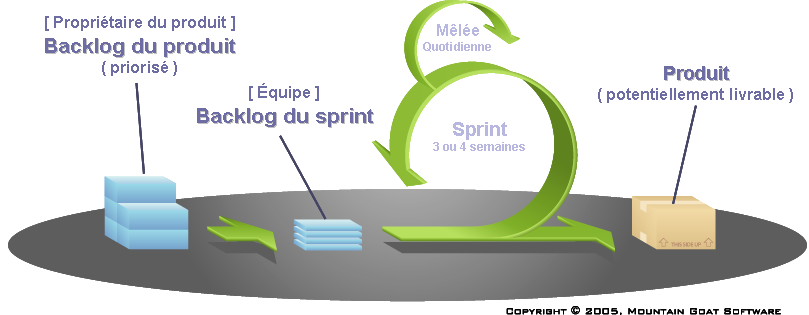
\includegraphics[width=\linewidth]{Images/scrum.png}
  \caption{Processus scrum}
  \label{fig:scrum}
\end{figure}
La planification du sprint correspond à lister les points prioritaires que l'équipe
pense pouvoir réaliser au cours d'un sprint.\\[0.2cm]
La revue du sprint a lieu en fin de sprint, l'équipe de développement présente les
fonctionnalités terminées au cours du sprint et recueille les retours du représentant des
utilisateurs finaux, c'est aussi à ce moment que la mise en place des prochains sprints peut être
anticipée.\\[0.2cm]
La Rétrospective de Sprint permet de faire un point sur le sprint en lui-même (productivité, efficacité, qualité…) afin de pouvoir s'améliorer pour les prochains sprints.\\[0.2cm]
Enfin la mêlée quotidienne permet de faire un point sur les avancements de chacun,
elle est courte et chacun réponds à trois questions principales : Qu'est-ce que j'ai terminé
depuis la dernière mêlée ? Qu'est-ce que j'aurai terminé d'ici la prochaine mêlée ? Quels
obstacles me retardent ?
\subsection{L'équipe SCRUM}
L’équipe a un rôle capital dans SCRUM : elle est constituée dans le but d’optimiser la flexibilité et la productivité; pour cela, elle s’organise elle-même et doit avoir toutes les compétences nécessaires au développement du produit. Elle est investie avec le pouvoir et l’autorité pour faire ce qu’elle a à faire.\\[0.5cm]
Scrum definit les rôles suivants :
\begin{description}
\item[Le Product Owner (le propriétaire du produit) : ] c’est une personne qui porte la vision du produit à réaliser, généralement c’est un expert dans le domaine.
\item[Le SCRUM Master (le directeur de produit) : ]c'est la personne qui doit assurer le bon déroulement des différents sprints du release, et qui doit impérativement maitriser SCRUM. 
\item[Le SCRUM Team (l’équipe de SCRUM) : ] constitué de personnes qui seront chargées d’implémenter les différents besoins du client. Bien évidemment, cette équipe sera constituée des développeurs, des testeurs, etc.
\end{description}
Dans le contexte de notre projet, Mr RHANIZAR est  le propriétaire du produit, et le directeur du produit puisqu’il satisfait les différents prés-requis de ces rôles cités précédemment et nous formons moi ELKAISSI SOUHAIL et CHATRIA ZAKARIA, les deux membres de l’équipe SCRUM. 
\section{Langage de modélisation}
Le langage de modélisation adopté durant ce stage sera le UML ,comme étant un outil comportant multiples points forts notamment sa standardisation ainsi que les divers diagrammes qu’il propose, et qui permettent la schématisation des systèmes complexes sous un format graphique et textuel simplifié et normalisé.\\
Généralement, le recours à la modélisation UML et plus particulièrement UML 2.0 procure de nombreux avantages qui agissent sur :
\begin{itemize}
\item La modularité.
\item L’abstraction.
\item La dissimulation.
\item La structuration cohérente des fonctionnalités et des données.
\end{itemize}
\section{TensorFlow : Librairie du machine learining et deep learning}
TensorFlow est une bibliothèque de logiciels open source pour le calcul numérique utilisant des graphes de flux de données. Il a été initialement développé par l'équipe Google Brain au sein de l'organisation de recherche Machine Intelligence de Google pour l'apprentissage automatique et la recherche sur les réseaux neuronaux profonds, mais le système est assez général pour être applicable dans une grande variété d'autres domaines. Il a atteint la version 1.0 en février 2017 et a poursuivi son développement rapide, avec plus de 21 000 engagements à ce jour, dont un grand nombre de contributeurs externes.\\[0.5cm]
TensorFlow est multi-plateforme. Il fonctionne sur presque tout : les processeurs graphiques et les processeurs normaux, y compris les plates-formes mobiles et embarquées, et même les unités de traitement tensoriel (TPU), qui sont des matériels spécialisés pour faire des calculs tensoriels. Ils ne sont pas encore largement disponibles, mais nous avons récemment lancé un programme alpha.

\section{Planification prévisionnelle}
\begin{tabular}{|p{6cm}|p{3cm}|p{3cm}|p{2cm}|}
\hline
\textbf{Nom de la tâche} & \textbf{Début de la tache} & \textbf{Date de la fin} & \textbf{Durée} \\
\hline
 Début du stage cadre & 23/04/2018 & 23/04/2018 & 1j\\
\hline
 Phase de preparation & 23/04/2018 & 01/05/2018 & 5j\\
\hline 
\textit{\hspace{1cm}Étude de la Solution actuelle} & \textit{22/04/2018} &  \textit{24/04/2018} & \textit{2j}\\
\hline
\textit{\hspace{1cm}Compréhension la totalité du projet} & \textit{25/04/2018} & \textit{01/05/2018} &  \textit{3j}\\
\hline
\textbf{Sprint 1: }Réalisation d'un modèle de prédiction avec l'algorithme CNN & 02/05/2018 & 23/05/2018 & 18j\\
\hline
Rédaction du Rapport partie 1 & 25/05/2018 & 25/05/2018 & 1j \\
\hline
\textbf{Sprint 2: }Réalisation d'un modèle de prédiction avec la méthode SVM & 26/05/2018 & 04/06/2018 & 7j\\
\hline
Rédaction du Rapport partie 2 & 05/06/2018 & 06/06/2018 & 2j \\
\hline
\textbf{Sprint 3: }Amélioration du modèle CNN en ajoutant une couche de word2vec & 07/06/2018 & 13/06/2018 & 8j\\
\hline
Rédaction du Rapport partie finale & 14/06/2018 & 16/05/2018 & 3j \\
\hline
Préparation de la soutenance & 17/06/2018 & 21/06/2018 & 5j \\
\hline 
Soutenance du Projet Cadre & 22/06/2018 & 22/06/2018 & 1j\\
\hline
\textbf{Sprint 4: }Réalisation d'un modèle hybride qui regroupe CNN avec word2vec et le SVM & 23/06/2018 & 06/07/2018 & 17j\\
\hline
\textbf{Sprint 5: }Déploiement de la solution finale & 09/07/2018 & 14/07/2018 & 5j\\
\hline
\end{tabular}
\begin{figure}[h]
  \caption{planification prévisionnelle}
  \label{fig:planification}
\end{figure}

\chapter{Analyse et Conception} % Main chapter title

\label{Chapitre 2} % For referencing the chapter elsewhere, use \ref{Chapter1} 

\lhead{Chapitre 2. \emph{Analyse et Conception}} % This is for the header on each page - perhaps a shortened title

%----------------------------------------------------------------------------------------

\section{Le Backlog du Produit}
Le backlog du produit est la liste des fonctionnalités attendues d'un produit. Plus exactement, au-delà de cet aspect fonctionnel, il contient tous les éléments qui vont nécessiter du travail pour l'équipe. Les éléments y sont classés par priorité ce qui permet de définir l'ordre de réalisation.\\[0.5cm]
Le backlog est élaboré avant le lancement des sprints, dans la phase de préparation (ou sprint 0). Il est utilisé pour planifier la release, puis à chaque sprint, lors de la réunion de planification du sprint pour décider du sous-ensemble qui sera réalisé.\\[0.2cm]
C'est donc un outil essentiel pour la planification. Mais il est aussi, par sa nature, un maillon de la gestion des exigences, puisqu'on y collecte ce que doit faire le produit.\\[0.2cm]
A tout moment, le backlog est visible par tout le monde.
\begin{figure}[h]
\begin{tabular}{|p{7cm}|p{4cm}|p{4cm}|}
\hline
\textbf{Story} & \textbf{Priorité2 } & \textbf{Effort ou chargen} \\
\hline
En tant qu'utilisateur, je souhaite pouvoir voir les news dans une fil d'actualité,et de sélectionner un contenu pour le visualiser. & \begin{center}M\end{center} & \begin{center}22\end{center}\\
\hline
En tant qu'utilisateur, je souhaite pouvoir ajouter un contenu au favoris pour que je puisse le visualiser plus tard. & \begin{center}C\end{center} & \begin{center}11\end{center}\\
\hline
En tant qu'utilisateur, je souhaite pouvoir visiter les différentes contenu par catégories,et de les sélectionner selon mon besoin. & \begin{center}M\end{center} & \begin{center}60\end{center}\\
\hline
\end{tabular}
  \caption{Le Backlog du Produit}
  \label{fig:Backlog}
\end{figure}
\subsection{La méthode de priorisation}
Pour prioriser le besoin, on a utilisé la méthode  \textbf{MoSCow} ; elle est une technique visant à prioriser des besoins ou des exigences en matière d'assistance à maîtrise d'ouvrage et de développement logiciel. L'objectif est que le maître d'œuvre et le maître d'ouvrage s'accordent sur l'importance des tâches à réaliser par rapport aux délais prévus.\\[0.2cm]
Les lettres majuscules de l'acronyme MoSCoW signifient (en anglais):\\[0.2cm]
\begin{description}
\item[M] must have this, c'est-à-dire 'doit être fait' (vital).
\item[S] should have this if at all possible, c'est-à-dire devrait être fait dans la mesure du possible (essentiel).
\item[C] could have this if it does not affect anything else, pourrait être fait dans la mesure où cela n'a pas d'impact sur les autres tâches (confort).
\item[W] won't have this time but would like in the future, ne sera pas fait cette fois mais sera fait plus tard' (luxe, c'est votre zone d'optimisation budgétaire).
\end{description}






\chapter{Sprint 0 : Preparation et étude de projet}
\label{Chapitre 3} % For referencing the chapter elsewhere, use \ref{Chapter1} 

\lhead{Chapitre 3. \emph{Sprint 0 : Preparation et étude de projet}} % This is for the header on each page - perhaps a shortened title

%----------------------------------------------------------------------------------------

\section{Spécification}
\subsection{Le Backlog du Sprint}


\begin{figure}[H]
\begin{tabular}{|p{7cm}|p{4cm}|p{4cm}|}
\hline
\textbf{Story} & \textbf{Priorité2 } & \textbf{Effort ou chargen} \\
\hline
En tant qu'utilisateur, je souhaite pouvoir voir les news dans une fil d'actualité,et de sélectionner un contenu pour le visualiser. & \begin{center}M\end{center} & \begin{center}22\end{center}\\
\hline
En tant qu'utilisateur, je souhaite pouvoir ajouter un contenu au favoris pour que je puisse le visualiser plus tard. & \begin{center}C\end{center} & \begin{center}11\end{center}\\
\hline
\end{tabular}
  \caption{Le Backlog du Sprint 0}
  \label{fig:Backlog}
\end{figure}
\section{Conception}
\subsection{Diagramme de cas d’utilisation : services client}
Comme on peut voir dans le digramme ci-dessous , on a trois acteurs : le client, l'administrateur, et le modèle de machine learning de classification.\\[0.2cm]
\begin{figure}[h]
	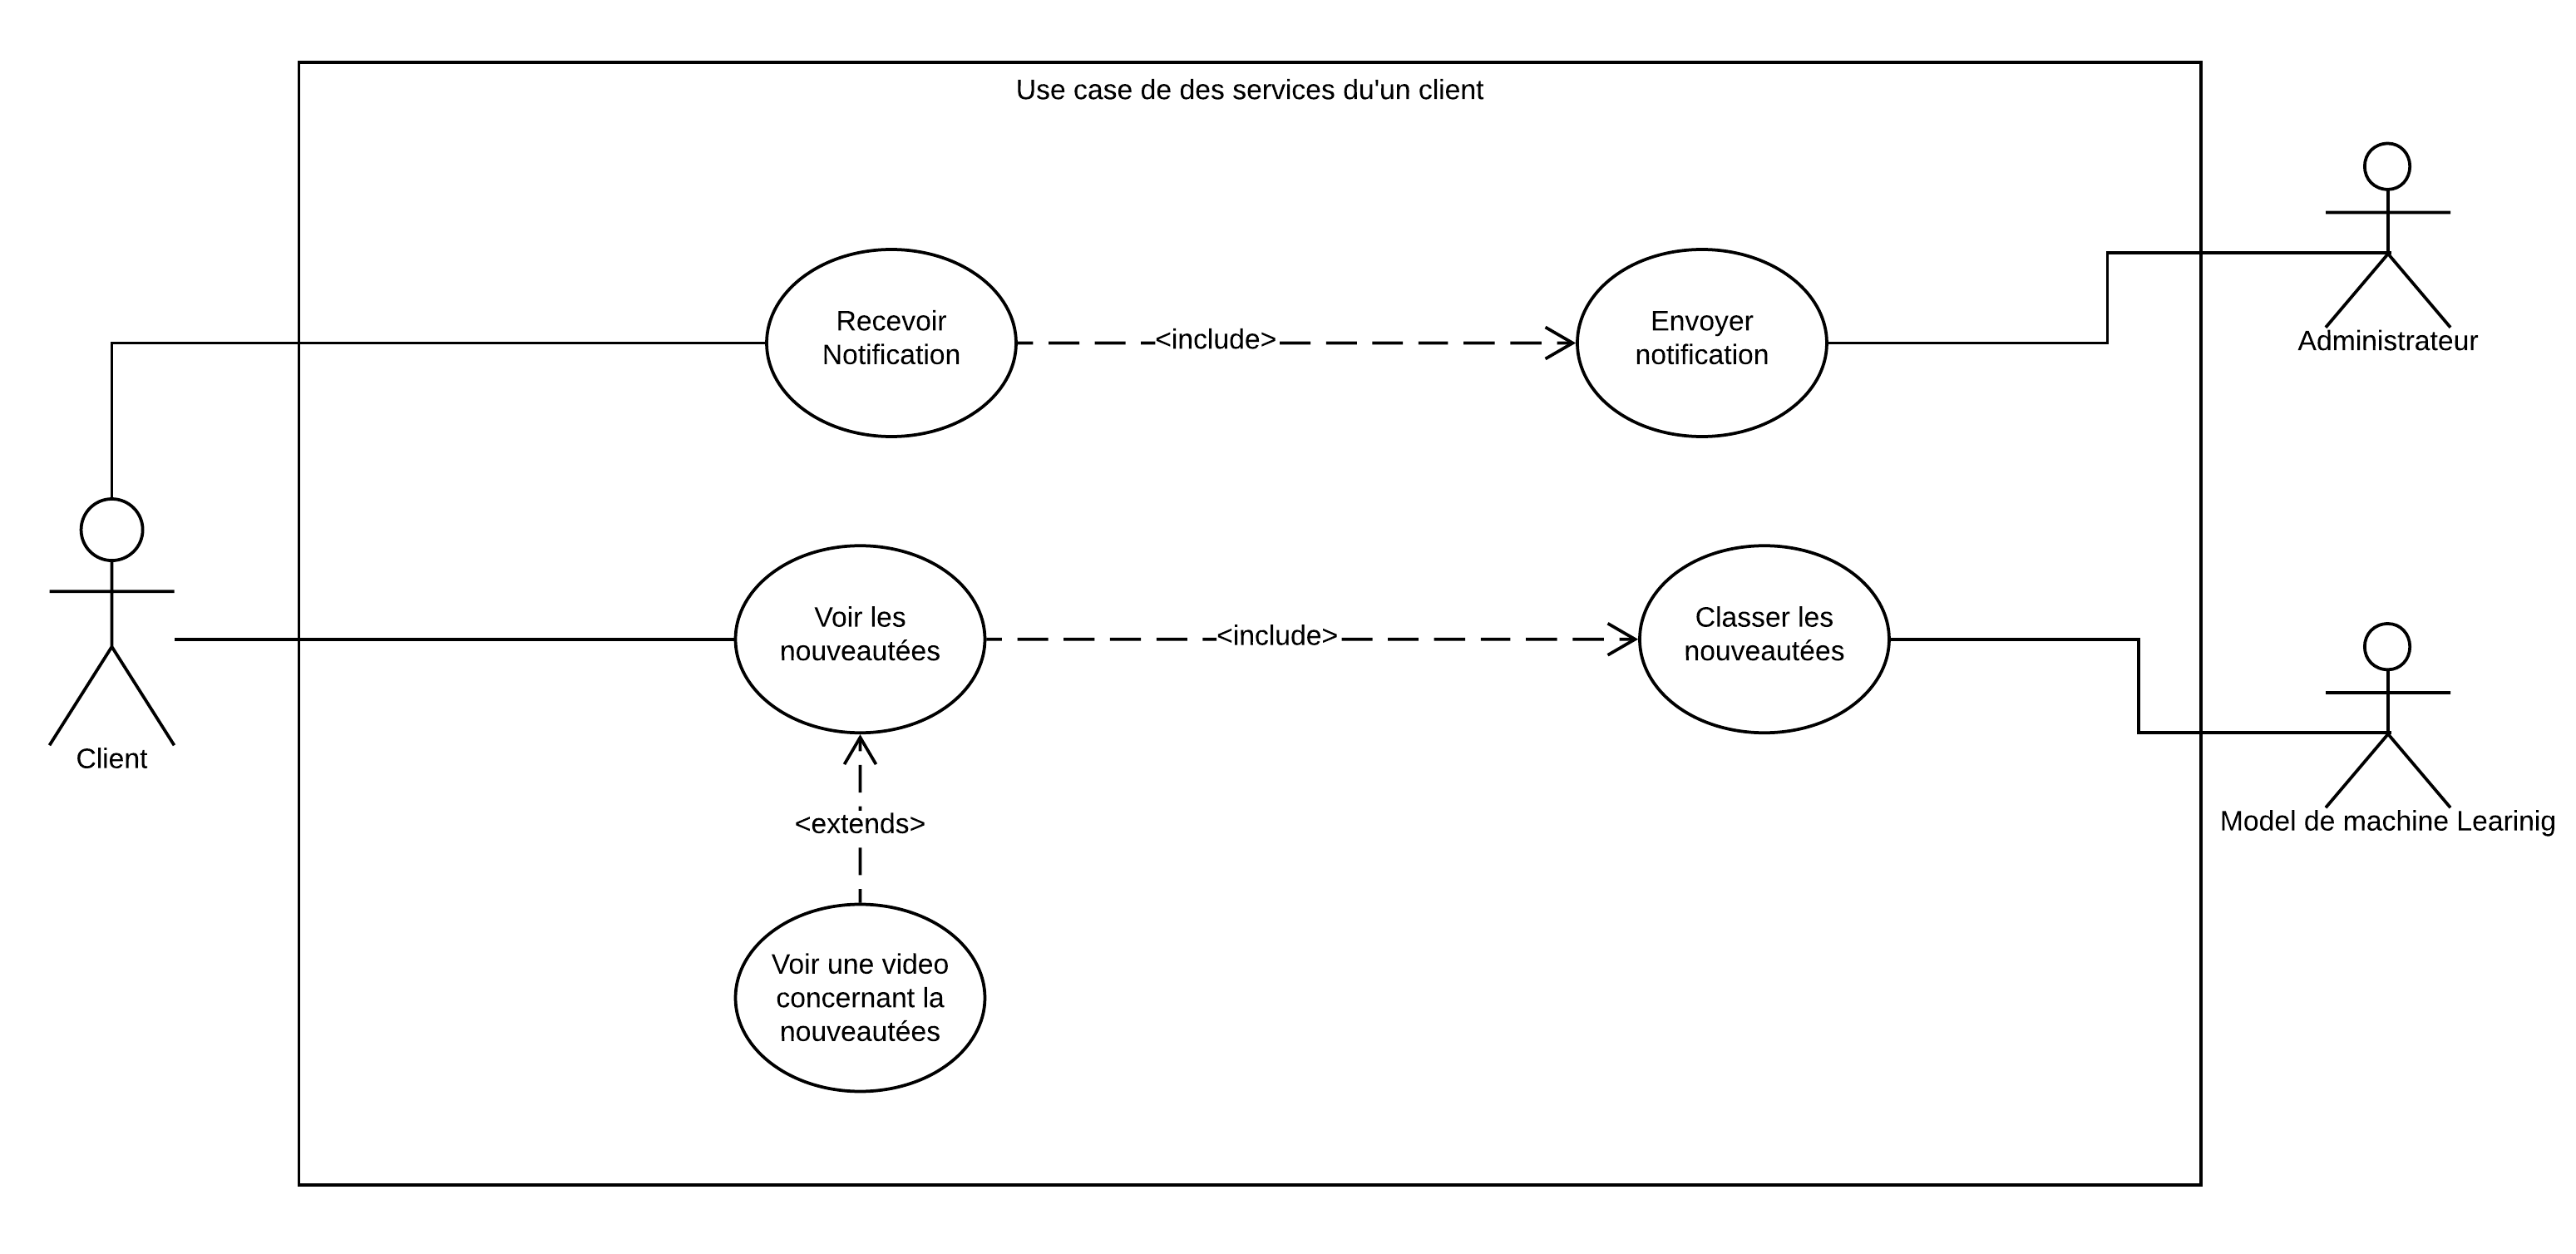
\includegraphics[width=\linewidth]{Images/use_case_sanadtech.png}
	\caption{Diagramme de cas d'utilisation}
	\label{fig:cas-utilisation}
\end{figure}

Pour que le client puisse visualiser les nouveautés , il faut que ces dernières soient classifier selon leurs catégories ,par le modèle, après cette manipulation ,le client pourra naviguer dans la page d'accueil et voir les nouveautés .\\[0.2cm]
Quand l'administrateur verra qu'une nouveauté est pertinente, il va lancer une notification, laquelle le client va recevoir, et pourra la visualiser en exclusivité.

\subsection{Diagramme de classes}
Comme on peut voir dans le digramme ci-dessous , on a cinq classes : User, News, Catégorie; ApiAtacker et le modèle.\\[0.2cm]
\begin{figure}[H]
	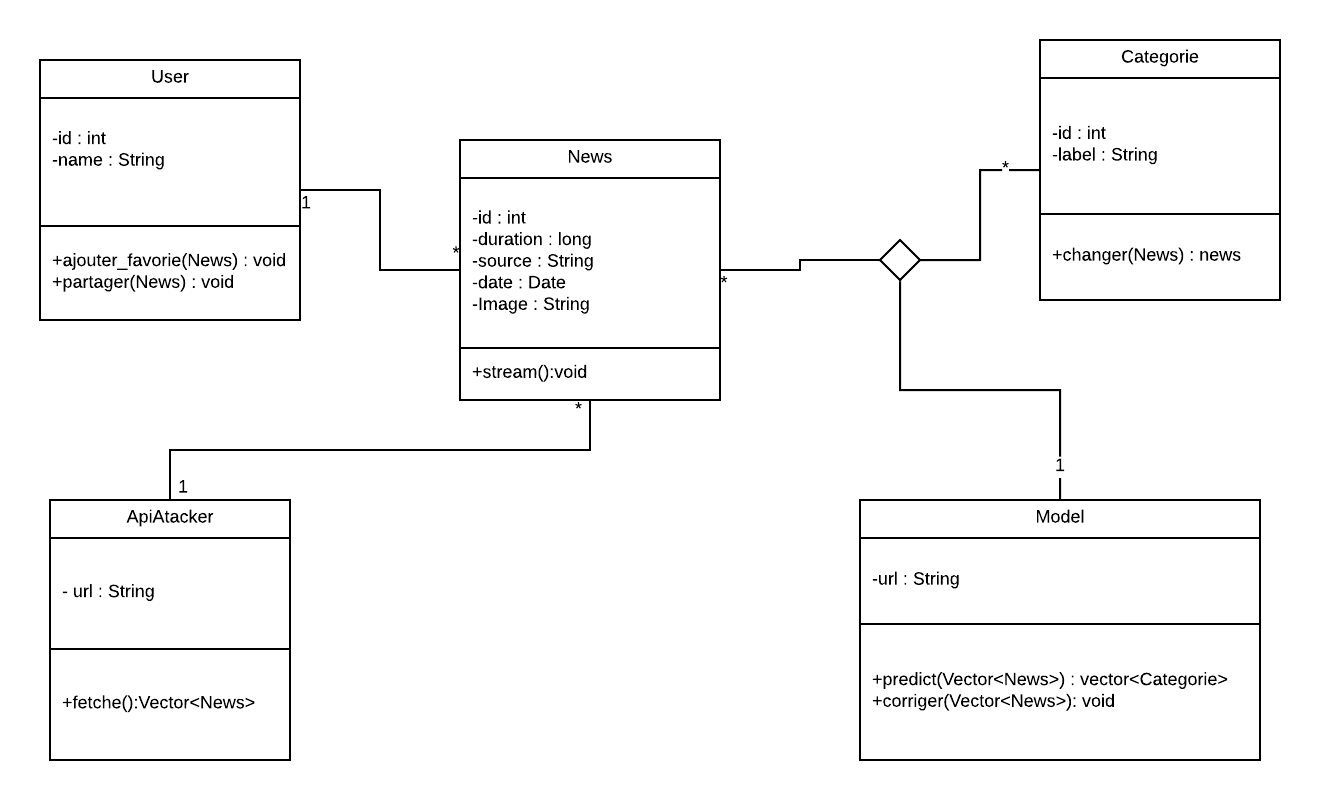
\includegraphics[scale=0.5]{Images/Class_diagram.png}
	\caption{Diagramme de classe}
	\label{fig:classe1}
\end{figure}

La classe \textbf{ApiAtacker},c'est la classe responsable de l'acquisition des données depuis les différentes sources qu'on a tels que : youtube, hesspress ...\\[0.2cm]
La classe News représente une nouveauté dans notre système, et chaque nouveauté est lié par une et une seul catégorie.\\[0.2cm]
Ici, la classe Model joue le rôle du classificateur, elle est celle qui transforme une nouveauté non étiqueté en une qui est qui est  étiqueté.\\[0.2cm]
Par ces différentes méthode, la classe User représente un client dans notre système, il décrit toutes ses actions possible.

\subsection{Diagramme de séquence}
Comme vous pouvez constater dans le diagramme ci-dessous, nous avons quatre ligne de vie, Client, Application front-end, Application back-end, Model tensorFlow.
\begin{figure}[H]
	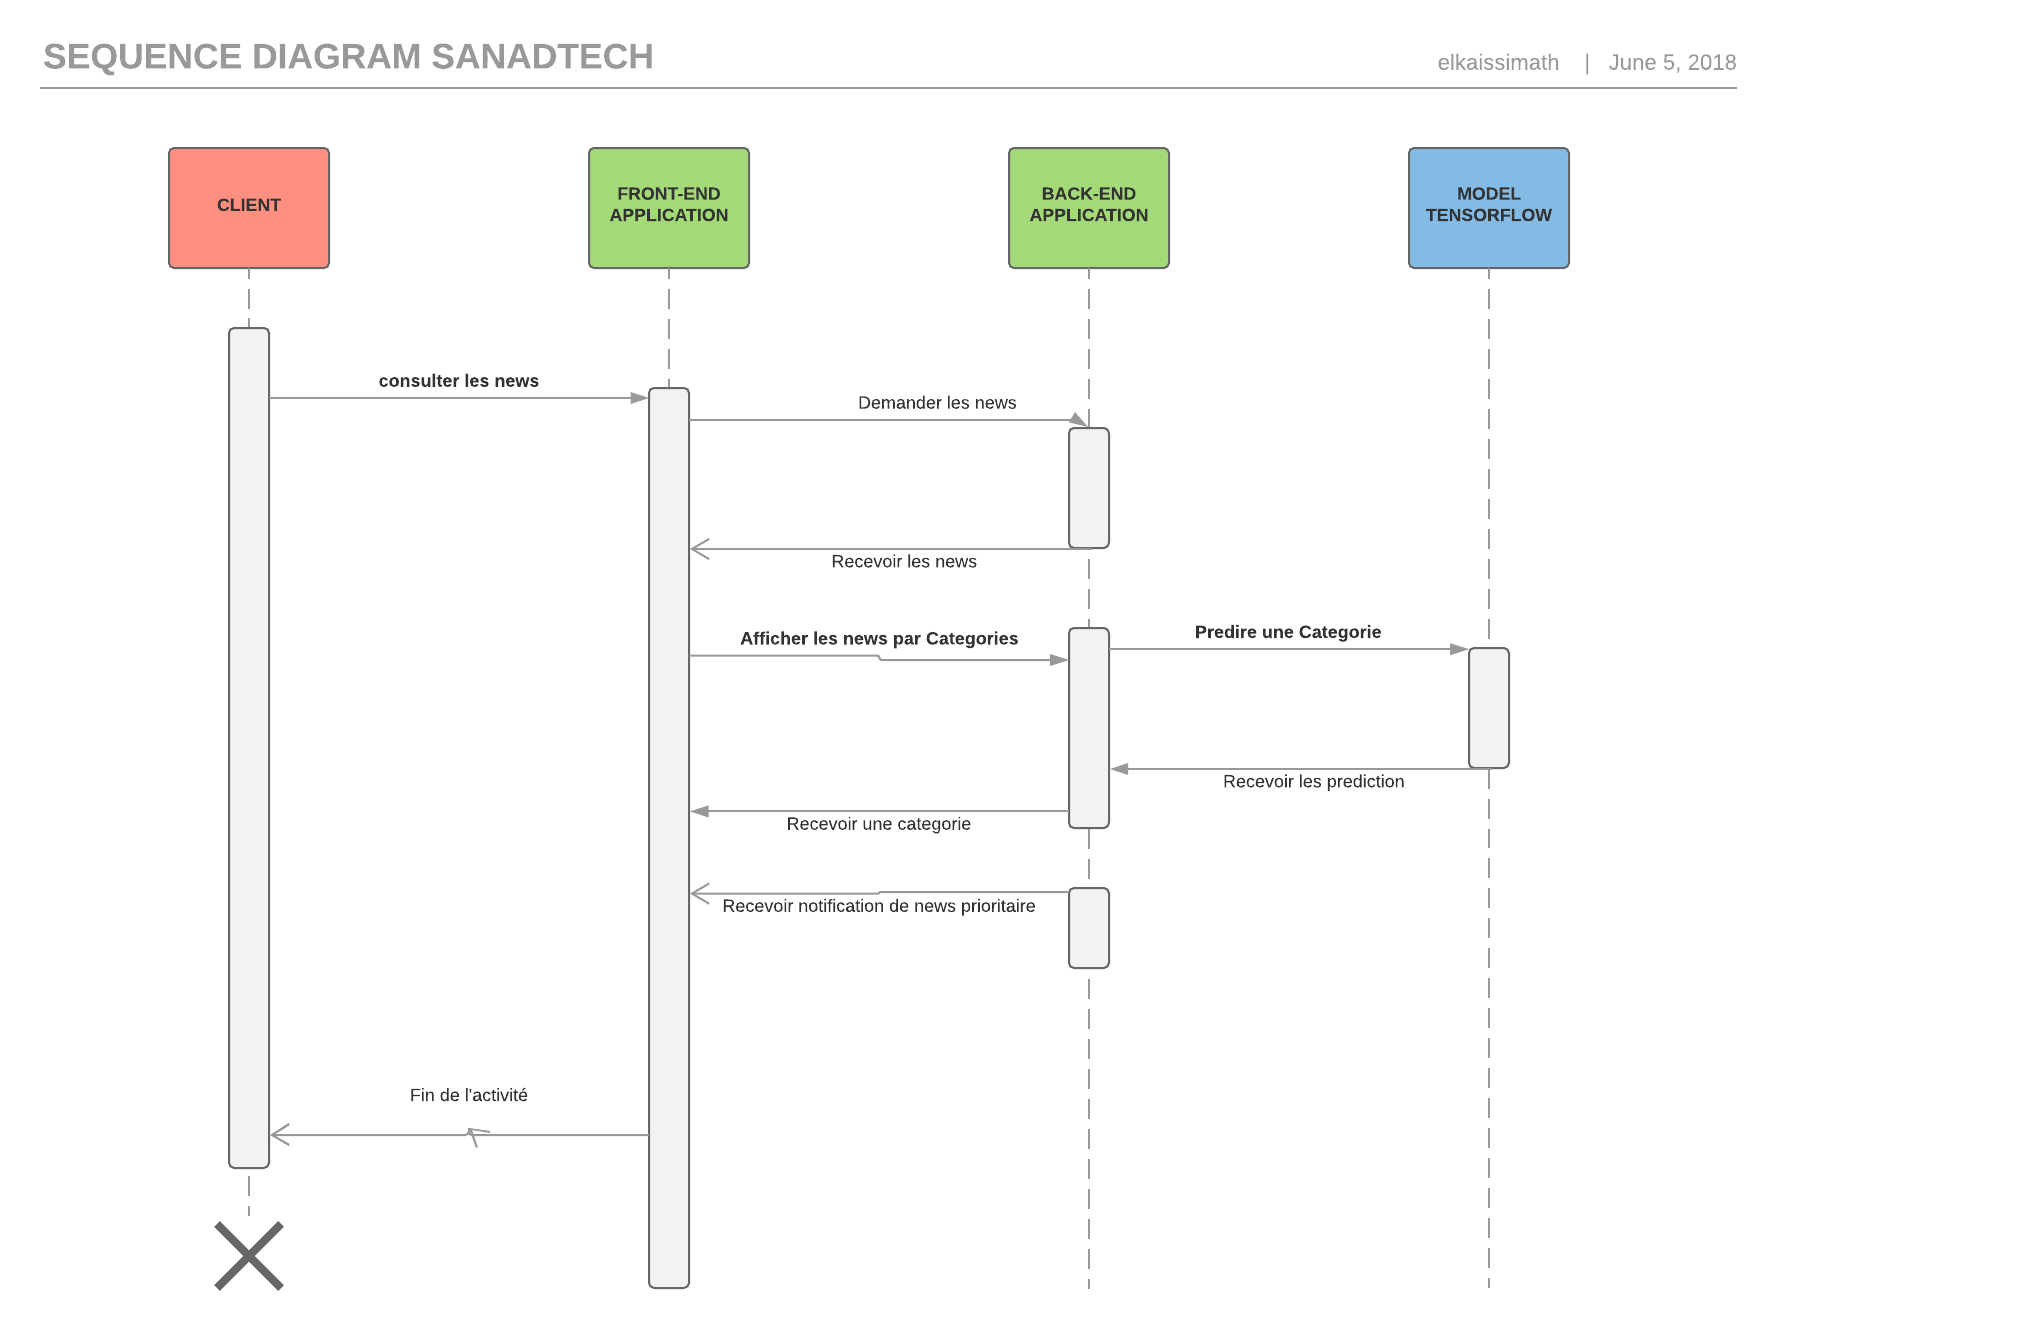
\includegraphics[width=\linewidth]{Images/Sequence_Diagram_Sanadtech.png}
	\caption{Diagramme de séquence}
	\label{fig:sequence}
\end{figure}
L'activité de l'application au point de vue client commence, qu'on un utilisateurs installe l'app dans son téléphone, il pourra ensuite recevoir les notifications des nouveautés les plus important.\\[0.2cm]
Quand un utilisateur consulte les nouveauté , le front-end envoi une requête au back-end, et ce dernier lui envoi tout les news par ordre de date.\\[0.2cm]
Si une news viens juste d'être intercepter par le back-end, il envoi alors, une requête au modèle Tensorflow pour savoir de quelle catégorie cette news appartiens. Et puis après, le back-end l'enregistre avec ça nouvelle classe ou catégorie.\\[0.4cm]
Si une nouveauté est jugé comme importante, elle sera envoyer vers toutes les utilisateurs sous la forme d'une notifications, depuis le back-end.\\[0.2cm]

\subsection{Diagramme de déploiement}
Le diagramme ci-dessous contient 4 nœuds principale, on site : front-end server, back-end server, database server , Model tensorflow server.
\begin{figure}[H]
	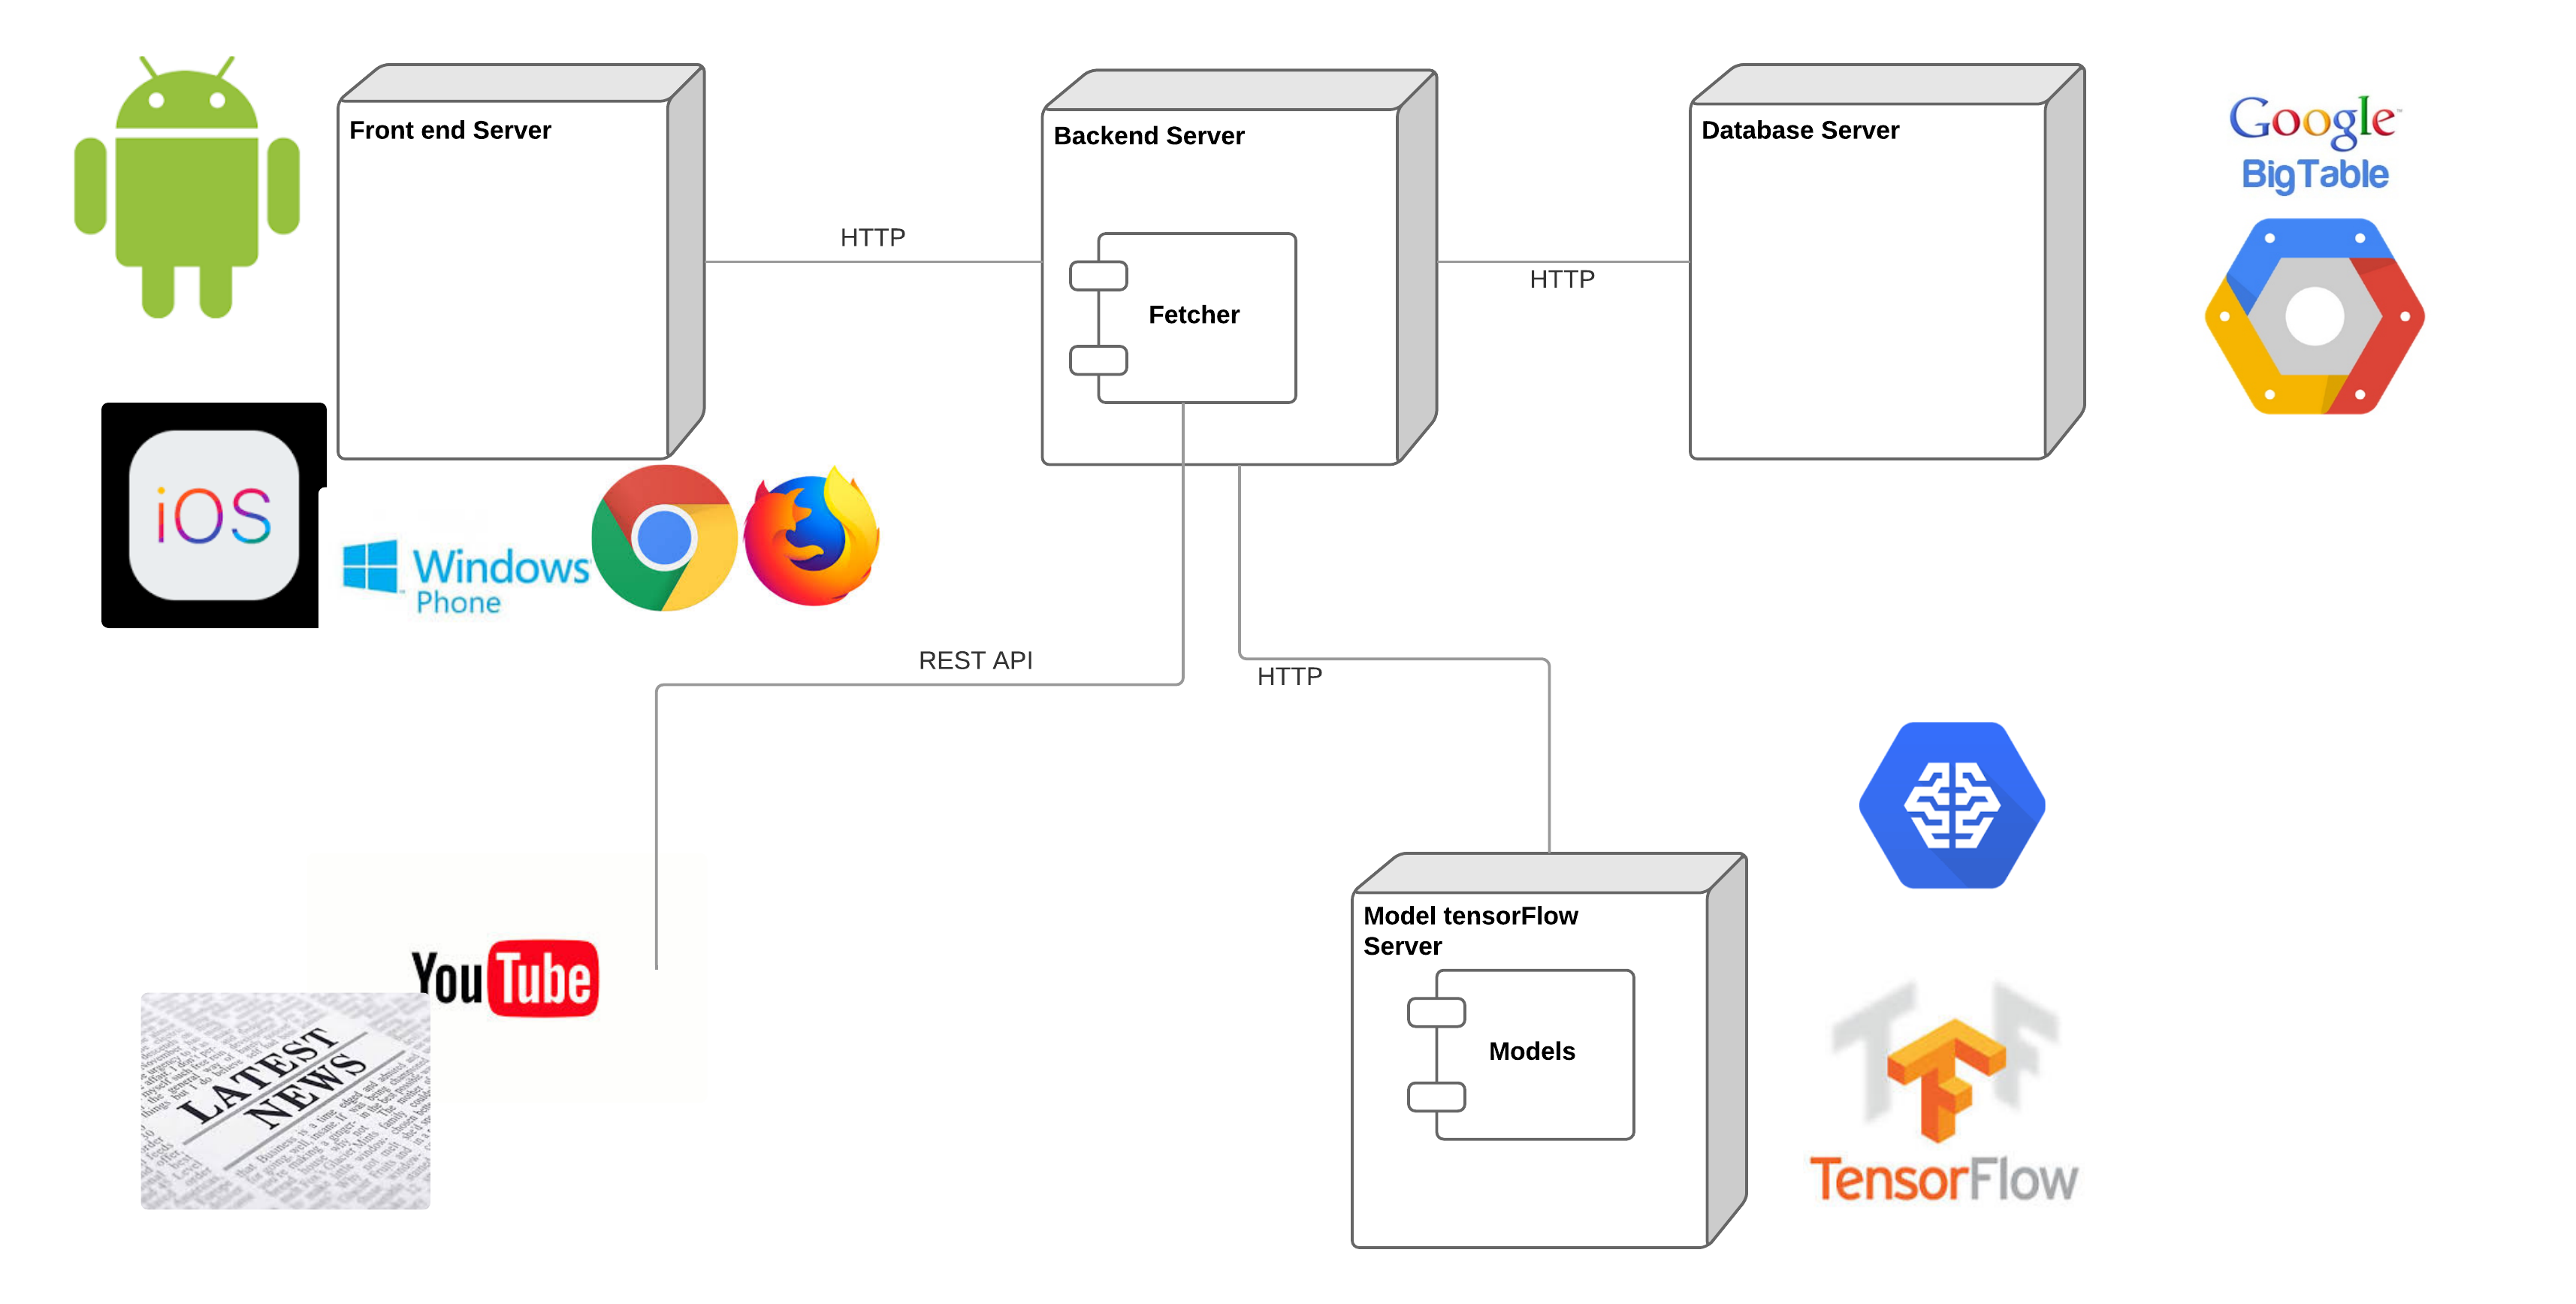
\includegraphics[width=\linewidth]{Images/Deployment_Diagram_Sanadtech.png}
	\caption{Diagramme de déploiement}
	\label{fig:deployment}
\end{figure}
Front-end server , c'est ou l'application finale est déployé, d'ici les utilisateur peuvent la télécharger, depuis les différentes Store, comme google play, apple store ...,ou la consulter dans le cas d'un navigateur.\\[0.2cm]
Back-end server, c'est ou le apiAtacker est situé , l'application envoi des requêtes vers ce nœud pour avoir les news.\\[0.2cm]
Database server, ici on stocke nos données , on utilise la base de donnée de google Big Table.\\[0.2cm]
Model Tensorflow Server, c'est ou notre model de prédiction est stocké , le modèle est écrit par tensorflow et déployer dans le service google ML-engine.



\section{NLP : Natural Language Processing}
Le modèle de classification qu'on va réaliser entre  dans la catégorie de la NLP, avant de le définir et l'expliquer, il faut d'abord rappeler qu'est ce que la machine learning et le deep learning.
\subsection{Machine learning}
L'apprentissage automatique (en anglais machine learning, littéralement « l'apprentissage machine ») ou apprentissage statistique, champ d'étude de l'intelligence artificielle, concerne la conception, l'analyse, le développement et l'implémentation de méthodes permettant à une machine (au sens large) d'évoluer par un processus systématique, et ainsi de remplir des tâches difficiles ou problématiques par des moyens algorithmiques plus classiques.\\[0.5cm]
L'analyse peut concerner des graphes, arbres, ou courbes (par exemple, la courbe d'évolution temporelle d'une mesure ; on parle alors de données continues, par opposition aux données discrètes associées à des attributs-valeurs classiques) au même titre que de simples nombres. Voir l'article Inférence bayésienne.\\[0.5cm]
Les algorithmes utilisés permettent, dans une certaine mesure, à un système piloté par ordinateur (un robot éventuellement), ou assisté par ordinateur, d'adapter ses analyses et ses comportements en réponse, en se fondant sur l'analyse de données empiriques provenant d'une base de données ou de capteurs.\\
La difficulté réside dans le fait que l'ensemble de tous les comportements possibles compte tenu de toutes les entrées possibles devient rapidement trop complexe à décrire (on parle d'explosion combinatoire). On confie donc à des programmes le soin d'ajuster un modèle pour simplifier cette complexité et de l'utiliser de manière opérationnelle. Idéalement, l'apprentissage visera à être non supervisé, c'est-à-dire que la nature des données d'entrainement n'est pas connue.\\[0.5cm]
Ces programmes, selon leur degré de perfectionnement, intègrent éventuellement des capacités de traitement probabiliste des données, d'analyse de données issues de capteurs, de reconnaissance (reconnaissance vocale, reconnaissance de forme, d'écriture…), de data-mining, d'informatique théorique…
\subsection{Depp Learning}
L'apprentissage profond1 (en anglais deep learning, deep structured learning, hierarchical learning) est un ensemble de méthodes d'apprentissage automatique tentant de modéliser avec un haut niveau d’abstraction des données grâce à des architectures articulées de différentes transformations non linéaires[réf. souhaitée]. Ces techniques ont permis des progrès importants et rapides dans les domaines de l'analyse du signal sonore ou visuel et notamment de la reconnaissance faciale, de la reconnaissance vocale, de la vision par ordinateur, du traitement automatisé du langage. Dans les années 2000, ces progrès ont suscité des investissements privés, universitaires et publics importants, notamment de la part des GAFA (Google, Apple, Facebook, Amazon).\\[0.5cm]
Les recherches dans ce domaine s’efforcent de construire de meilleures représentations du réel et de créer des modèles capables d’apprendre ces représentations à partir de données non labellisées à grande échelle. Certaines de ces représentations s’inspirent des dernières avancées en neuroscience. Il s'agit, grosso modo, d'interprétations du traitement de l’information et des modèles de communication du système nerveux, à l'image de la façon dont le système nerveux établit des connexions en fonction des messages reçus, de la réponse neuronale et du poids des connexions entre les neurones du cerveau.\\
Les différentes architectures de « deep learning » telles que les « deep neural networks », les « convolutional deep neural networks », et les « deep belief network » ont plusieurs champs d’application :
\begin{itemize}
\item la vision par ordinateur (reconnaissance de formes) ;
\item la reconnaissance automatique de la parole ;
\item le traitement automatique du langage naturel ;
\item la reconnaissance audio et la bio-informatique.
\end{itemize}
Dans ces deux derniers domaines, notamment, elles ont obtenu des résultats très prometteurs.
\subsection{NLP}
Le traitement automatique du langage naturel (abr. TALN), ou traitement automatique de la langue naturelle1, est un domaine multidisciplinaire impliquant la linguistique, l'informatique et l'intelligence artificielle. Il vise à créer des outils de traitement de la langue naturelle pour diverses applications. Il ne doit pas être confondu avec la linguistique informatique, qui vise à comprendre les langues au moyen d'outils informatiques.\\[0.5cm]
Le TALN est sorti des laboratoires de recherche pour être progressivement mis en œuvre dans des applications informatiques nécessitant l'intégration du langage humain à la machine2. Aussi le TALN est-il parfois appelé ingénierie linguistique3. En France, le traitement automatique de la langue naturelle a sa revue, ATALA, publiée par l’Association pour le traitement automatique des langues.




\section{Préparation des données}	
Dans un projet de machine learning, il est important de bien encadrer les données, parce que en sens large, il constitue l'enjeu majeur. Pour ce fait, on a suivi ces principaux étapes :
\subsection{Identification des sources de données}
Les données qu'on traite sont des données de type chaine de caractère qui comporte deux champs, le première champs et celui de la catégorie ou la classe, et le deuxième champs et celui de la description ou le titre de la vidéo.
\begin{figure}[H]
	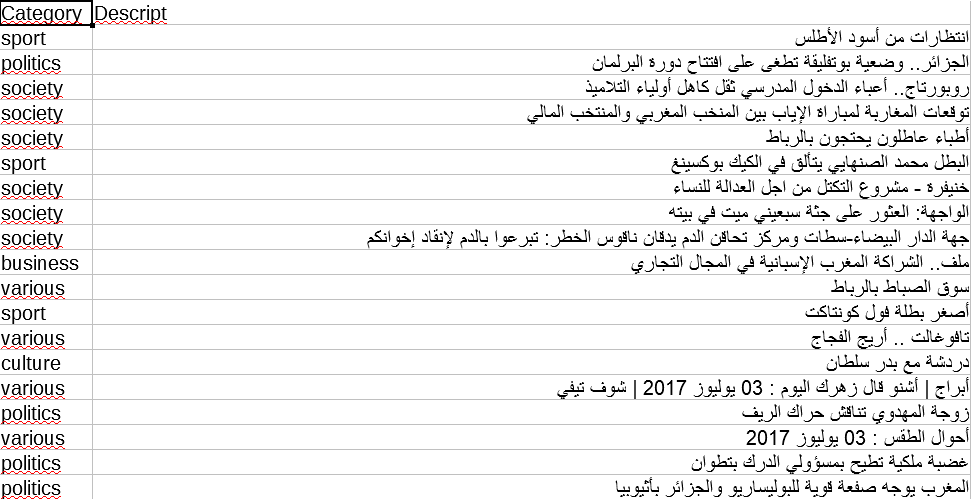
\includegraphics[width=\linewidth]{Images/donnees_contenu.png}
	\caption{Exemple de données}
	\label{fig:donnees}
\end{figure}	
Le format des données actuellement, avec lequelle on va faire l'entrainement et les testes, sont en format \textbf{CSV}, l'avantage de ce format c'est qu'il est facilement manipulable par le langage de programmation python même si la taille de données peut être grande.\\[0.2cm]
On récupère ses données là depuis plusieurs source, et après on extrait les données juger utiles pour les prédiction, dans ce cas les description des vidéo.
\subsection{Définition du lieu d'entreposage}
Les données transformé doivent etre stockés, pour le fait de ne pas les predire une deuxieme fois, on utilise dans notre projet la base données google, Big Table, il  est un système de gestion de base de données compressées, haute performance, et propriétaire, C'est une base de données orientée colonnes, dont se sont inspirés plusieurs projets libres, comme HBase, Cassandra ou Hypertable.\\
\begin{figure}[H]
	\begin{center}
	
\includegraphics[width=100mm,scale=0.5]{Images/google-cloud-bigtable.png}
	\end{center}
	\caption{google cloud big table}
	\label{fig:gglcloudbigtable}
\end{figure}	
 Google ne distribue pas sa base de données mais propose une utilisation publique de BigTable via sa plateforme d'application Google App Engine.
\subsection{Nettoyage des données}
Les données utilisées proviennent de diverses sources et processus et peuvent contenir des irrégularités ou des données corrompues compromettant la qualité de l'ensemble de données. Les problèmes typiques de qualité des données qui se posent sont les suivants:
\begin{description}
\item[Incomplet : ] Les données manquent d'attributs ou contiennent des valeurs manquantes.
\item[Noisy : ]les données contiennent des enregistrements erronés ou des valeurs aberrantes.
\item[Inconsistant : ]les données contiennent des enregistrements ou des divergences conflictuels.
\end{description}
Les données de qualité sont une condition préalable à la qualité des modèles prédictifs. Pour éviter les «déchets» et améliorer la qualité des données et donc la performance du modèle, nous avons trouvé qu'il est impératif de réaliser un écran d'intégrité des données afin de repérer rapidement les problèmes de données et de décider des étapes de traitement et de nettoyage correspondantes.
\subsection{Features generation}
C'est un processus consistant à prendre des données brutes non structurées et à définir des caractéristiques (c'est-à-dire des variables) pour une utilisation potentielle dans l'analyse statistique.\\
 Par exemple, dans le cas de l'exploration de texte \textit{(notre cas)}, on a  commencé avec un journal brut de milliers de descriptions \textit{(celles des vidéos)} et générer des fonctionnalités en supprimant des mots de faible valeur. des blocs de mots \textit{(n-grammes)} ou en appliquant d'autres règles.
\subsection{Feature extration}
Une fois les fonctionnalités générées, il est souvent nécessaire de tester les transformations des entités d'origine et de sélectionner un sous-ensemble de ce groupe de caractéristiques potentielles originales et dérivées à utiliser dans notre modèle (extraction et sélection de caractéristiques).\\[0.2cm]
Tester des valeurs dérivées est une étape courante car les données peuvent contenir des informations importantes qui ont un modèle ou une relation non linéaire avec notre résultat, ainsi l'importance de l'élément de données peut seulement apparaître dans son état transformé (par exemple des dérivés d'ordre supérieur).\\[0.2cm]
 L'utilisation d'un trop grand nombre de caractéristiques peut entraîner une colinéarité multiple ou confondre des modèles statistiques, alors qu'extraire le nombre minimum de caractéristiques correspondant au but de votre analyse suit le principe de la parcimonie.

\chapter{Sprint 1 : Réalisation d’un modèle de prédiction avec l’algorithme CNN}
\label{Chapitre 4} % For referencing the chapter elsewhere, use \ref{Chapter1} 

\lhead{Chapitre 4. \emph{Sprint 1 : Réalisation d’un modèle de prédiction avec l’algorithme CNN}} % This is for the header on each page - perhaps a shortened title

%----------------------------------------------------------------------------------------
\section{Spécification}
\subsection{Le Backlog du Sprint}
\begin{figure}[H]
\begin{tabular}{|p{7cm}|p{4cm}|p{4cm}|}
\hline
\textbf{Story} & \textbf{Priorité2 } & \textbf{Effort ou chargen} \\
\hline
En tant qu'utilisateur, je souhaite pouvoir visiter les différentes contenu par catégories,et de les sélectionner selon mon besoin. & \begin{center}M\end{center} & \begin{center}22\end{center}\\
\hline
\end{tabular}
  \caption{Le Backlog du Sprint 1}
  \label{fig:Backlog1}
\end{figure}


\section{Conception}

\subsection{Qu'est ce qu'un CNN/RNN ?}
\textbf{Réseau de neurones convolutifs}\\[0.5cm]
En apprentissage automatique, un réseau de neurones convolutifs ou réseau de neurones à convolution (en anglais CNN ou ConvNet pour Convolutional Neural Networks) est un type de réseau de neurones artificiels acycliques (feed-forward), dans lequel le motif de connexion entre les neurones est inspiré par le cortex visuel des animaux. Les neurones de cette région du cerveau sont arrangés de sorte qu'ils correspondent à des régions qui se chevauchent lors du pavage du champ visuelle.\\[0.2cm]
 Leur fonctionnement est inspiré par les processus biologiques, ils consistent en un empilage multicouche de perceptrons, dont le but est de pré-traiter de petites quantités d'informations. Les réseaux neuronaux convolutifs ont de larges applications dans la reconnaissance d'image et vidéo, les systèmes de recommandation et le traitement du langage naturel.\\[1cm]

 \textbf{Réseau de neurones récurrents}\\[0.5cm]
 
 Un réseau de neurones récurrents est un réseau de neurones artificiels présentant des connexions récurrentes. Un réseau de neurones récurrents est constitué d'unités (neurones) inter-connectés interagissant non-linéairement et pour lequel il existe au moins un cycle dans la structure. Les unités sont reliées par des arcs (synapses) qui possèdent un poids. La sortie d'un neurone est une combinaison non linéaire de ses entrées.\\[0.2cm]
Les réseaux de neurones récurrents sont adaptés pour des données d'entrée de taille variable. Ils conviennent en particulier pour l'analyse de séries temporelles. Ils sont utilisés en reconnaissance automatique de la parole ou de l'écriture manuscrite - plus en général en reconnaissance de formes - ou encore en traduction automatique. « Dépliés », ils sont comparables à des réseaux de neurones classiques avec des contraintes d'égalité entre les poids du réseau (voir schéma ci-dessous).

\begin{figure}[H]
	\begin{center}
	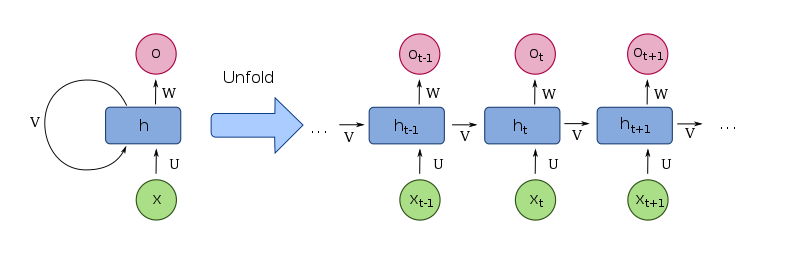
\includegraphics[width=100mm,scale=0.5]{Images/rnn.png}
	\end{center}
	\caption{Schéma d'un réseau de neurones récurrents à une unité reliant l'entrée et la sortie du réseau. A droite la version « dépliée » de la structure.}
	\label{fig:rnn}
\end{figure}


\subsection{L'architecture de notre réseaux neuronal}
Le réseaux neuronal qu'on a adopté est comme suite : 

\begin{figure}[H]
	\begin{center}
	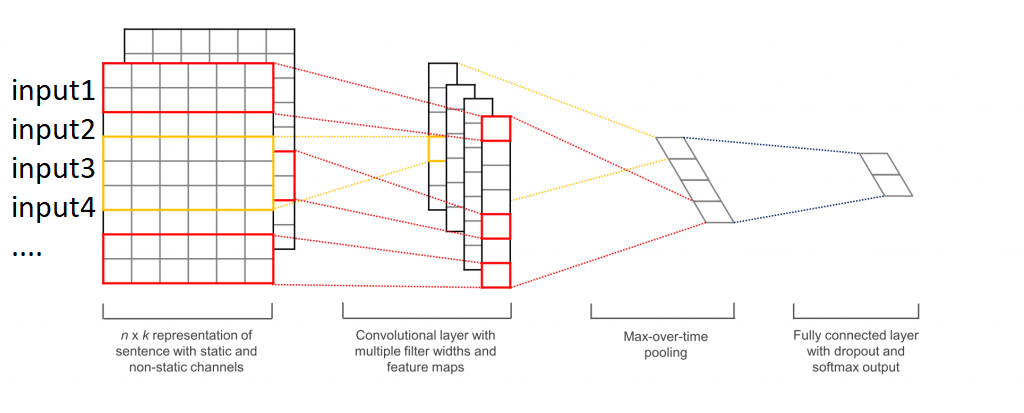
\includegraphics[width=\linewidth]{Images/cnn.png}
	\end{center}
	\caption{La structure du reseaux neuronal ,réaliser par cnn.}
	\label{fig:cnn1}
\end{figure}

Les premières couches incorpore des mots dans des vecteurs de basse dimension. La couche suivante effectue des convolutions sur les vecteurs de mots incorporés, en utilisant des tailles de filtres multiples.\\[0.2cm]

\begin{figure}[H]
	\begin{center}
	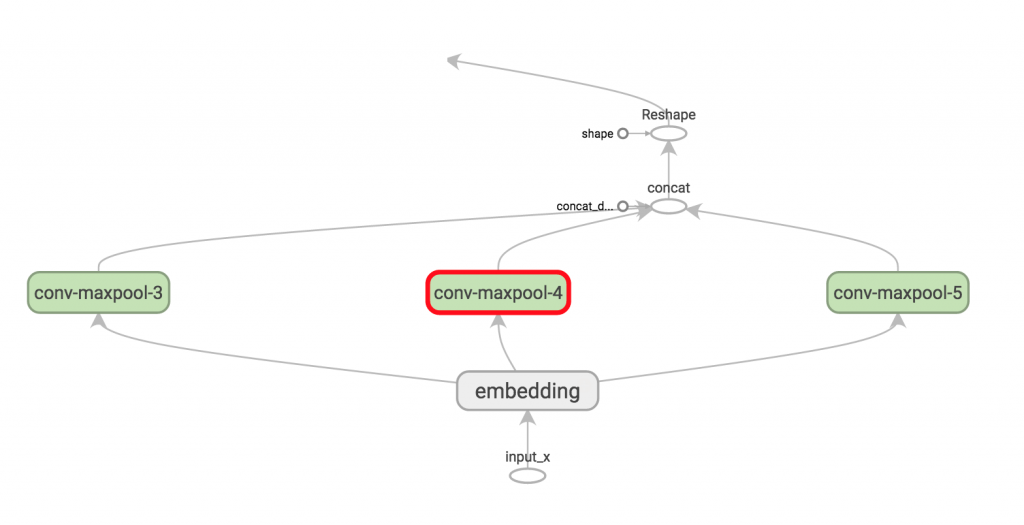
\includegraphics[width=\linewidth]{Images/cnn1.png}
	\end{center}
	\caption{La structure du réseaux neuronal, structure des couches de convolutions.}
	\label{fig:cnn1}
\end{figure}
 Par exemple, glisser sur 3, 4 ou 5 mots à la fois. Ensuite, nous max-poolons le résultat de la couche convolutionnelle dans un long vecteur de caractéristiques,et on ajoute une régularisation de décrochage, et en fin on  classe le résultat en utilisant une couche softmax.\\[0.5cm]
 
Puisque on ne peut pas traiter les chaînes de caractères dans un réseaux neuronal, on doit transformer ces données là, en des données numérique, c’est pour cela, j’ai utilisé une transformation classique « Embeding» qui mappe chaque mot qui existe dans mon dictionnaire de mot ,en des numéro significatif.\\[0.2cm]
Pour bien comprendre le déroulement ,et le processus de fonctionnement de ce réseaux neuronal , voici une figure descriptive :

\begin{figure}[H]
	\begin{center}
	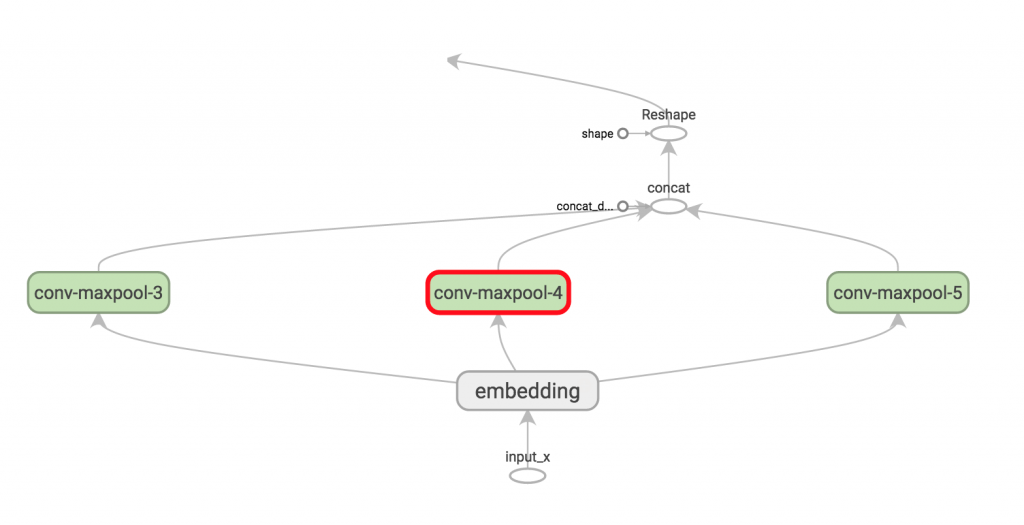
\includegraphics[width=\linewidth]{Images/cnn1.png}
	\end{center}
	\caption{Architecture des couches du réseaux neuronal.}
	\label{fig:cnn2}
\end{figure}

Ici, \textbf{W} est notre matrice de filtre et h est le résultat de l'application de la non-linéarité à la sortie de la convolution. Chaque filtre glisse sur l'ensemble de l'incorporation, mais varie en nombre de mots. Le remplissage \textit{VALIDE} signifie que nous glissons le filtre sur notre phrase sans capitonner les bords, en effectuant une convolution étroite qui nous donne une sortie de forme $ [1, sequenceLengthFilterSize+1, 1, 1] $.\\[0.2cm]
 L'exécution de \textbf{max-pooling} sur la sortie d'une taille de filtre spécifique nous laisse avec un tenseur de forme $ [batchSize, 1, 1, numFilters] $. C'est essentiellement un vecteur de caractéristiques, où la dernière dimension correspond à nos caractéristiques.\\[0.2cm]
Une fois que nous avons tous les tenseurs de sortie regroupés de chaque taille de filtre, nous les combinons en un long vecteur de forme de forme $ [tailleBatch, numFiltersTotal] $. \\[0.2cm]
L'utilisation de -1 dans tf.reshape indique à TensorFlow d'aplatir la cote lorsque cela est possible.\\[0.2cm]

Pour régulariser notre CNN, j’ai utilisé une couche \textbf{Dropout} ,l'idée derrière  est simple. Une couche de décrochement stochastique \textbf{désactive} une fraction de ses neurones. Cela empêche les neurones de co-adapter, et les oblige à apprendre des fonctionnalités utiles individuellement.\\[0.2cm]
 La fraction de neurones que nous gardons activée est définie sur notre réseau. Nous avons réglé ceci à quelque chose comme \textit{0.5} pendant l'entraînement, et à \textit{1} (désactiver la couche) pendant l'évaluation.\\[0.2cm]
 
 En utilisant le vecteur de caractéristiques de \textbf{max-pooling} (avec \textbf{dropout} appliqué), nous pouvons générer des prédictions en faisant une multiplication matricielle et en choisissant la classe ayant le score le plus élevé. Nous pourrions également appliquer une fonction \textbf{softmax} pour convertir les scores bruts en probabilités normalisées, mais cela ne changerait pas nos prédictions finales.\\[0.2cm]
 
 En utilisant nos \textit{scores}, nous pouvons définir la fonction de perte. La perte est une mesure de l'erreur que notre réseau fait, et notre objectif est de le minimiser. La fonction de perte standard pour la catégorisation pose des problèmes de perte d'\textit{entropie} croisée.\\[0.5cm]
Enfin le graphe final résultant ressemble à ça :
\begin{figure}[H]
	\begin{center}
	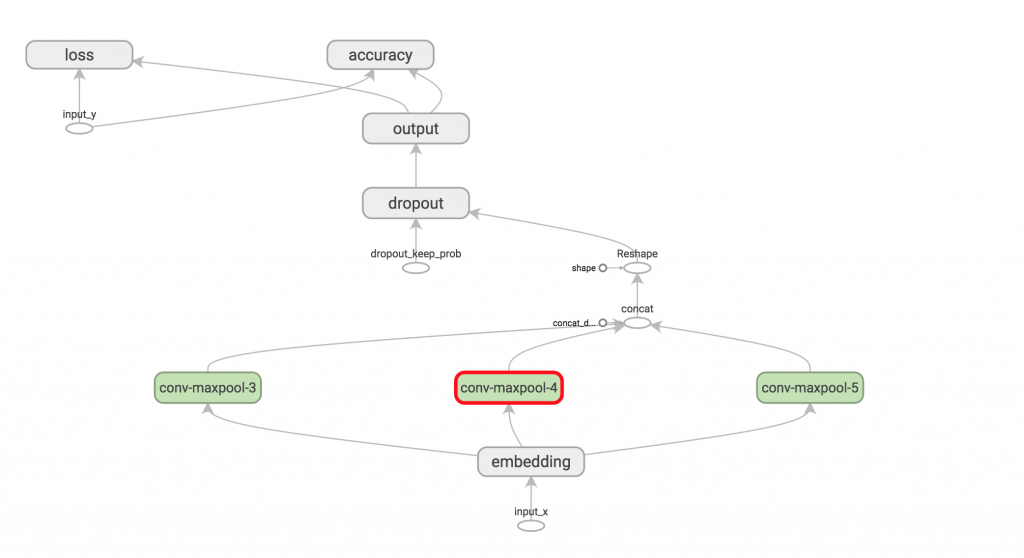
\includegraphics[width=\linewidth]{Images/cnn3.png}
	\end{center}
	\caption{Graphe qui représente les étapes du traitement du modèle.}
	\label{fig:rnn}
\end{figure}


 L’état des pertes sur les variables de décision :

\begin{figure}[H]
	\begin{center}
	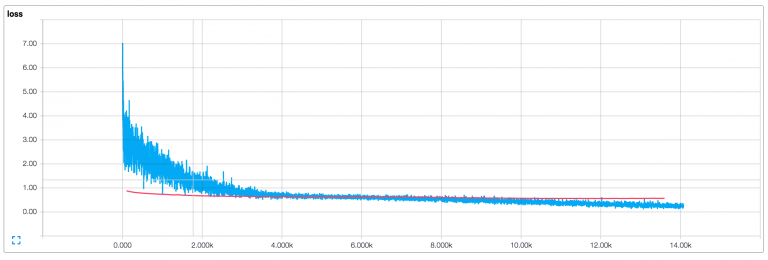
\includegraphics[width=\linewidth]{Images/cnn4.png}
	\end{center}
	\caption{Graphe qui représente les données perdues, du reseaux CNN/RNN.}
	\label{fig:rnn}
\end{figure}
 l'état des précision qui est égale à 0,76:
\begin{figure}[H]
	\begin{center}
	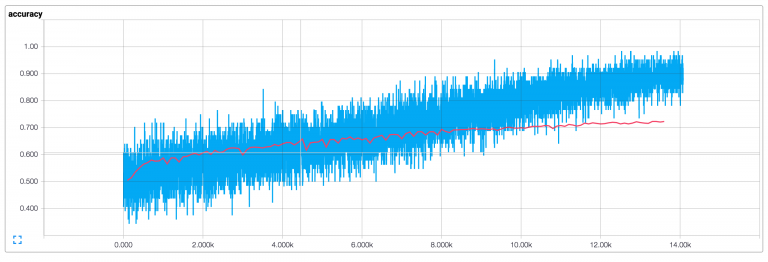
\includegraphics[width=\linewidth]{Images/cnn5.png}
	\end{center}
	\caption{Graphe qui représente la précision, du reseaux CNN/RNN}
	\label{fig:rnn}
\end{figure}




\chapter{Sprint 2 : Réalisation d’un modèle de prédiction avec l’algorithme SVM}
\label{Chapitre 5} % For referencing the chapter elsewhere, use \ref{Chapter1} 

\lhead{Chapitre 5. \emph{Sprint 2 : Réalisation d’un modèle de prédiction avec l’algorithme SVM}} % This is for the header on each page - perhaps a shortened title

%----------------------------------------------------------------------------------------
\section{Spécification}
\subsection{Le Backlog du Sprint}
\begin{figure}[H]
\begin{tabular}{|p{7cm}|p{4cm}|p{4cm}|}
\hline
\textbf{Story} & \textbf{Priorité2 } & \textbf{Effort ou chargen} \\
\hline
En tant qu'utilisateur, je souhaite pouvoir visiter les différentes contenu par catégories,et de les sélectionner selon mon besoin. & \begin{center}M\end{center} & \begin{center}22\end{center}\\
\hline
\end{tabular}
  \caption{Le Backlog du Sprint 2}
  \label{fig:Backlog2}
\end{figure}
\section{Conception}
\subsection{Qu'est ce que le SVM ?}
Les machines à vecteurs de support ou séparateurs à vaste marge (en anglais support vector machine, SVM) sont un ensemble de techniques d'apprentissage supervisé destinées à résoudre des problèmes de discrimination 1 et de régression. Les SVM sont une généralisation des classifieurs linéaires.\\[0.5cm]
Les séparateurs à vaste marge ont été développés dans les années 1990 à partir des considérations théoriques de Vladimir Vapnik sur le développement d'une théorie statistique de l'apprentissage : la théorie de Vapnik-Chervonenkis. Ils ont rapidement été adoptés pour leur capacité à travailler avec des données de grandes dimensions, le faible nombre d'\textbf{hyperparamètres}, leurs garanties théoriques, et leurs bons résultats en pratique.\\[0.5cm]
\begin{figure}[H]
	\begin{center}
	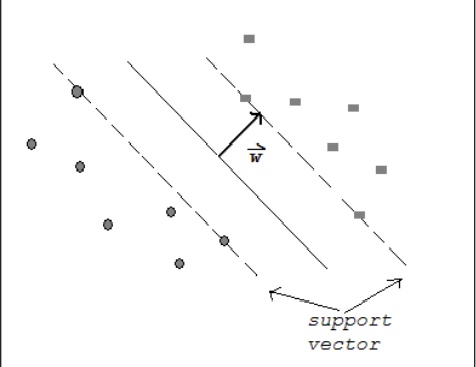
\includegraphics[scale=0.5]{Images/ex_svm.png}
	\end{center}
	\caption{Exemple d'un hyperplan pattern de SVM}
	\label{fig:svm0}
\end{figure}
Les SVM ont été appliqués à de très nombreux domaines (bio-informatique, recherche d'information, vision par ordinateur, finance…). Selon les données, la performance des machines à vecteurs de support est de même ordre, ou même supérieure, à celle d'un réseau de neurones ou d'un modèle de mélanges gaussiens.\\[1cm]
Les machines à vecteurs de support sont basées sur le principe de la structure de minimisation de risque, dans la théorie de l'apprentissage aléatoire.L'idée de la structure de minimisation de risque est de trouver une hypothèse \textbf{\textit{h}} avec laquelle on peut garantir, d'avoir le plus petit cout d'erreur. \\La vrai erreur de \textbf{\textit{h}}, c'est la probabilité que \textbf{\textit{h}} va faire une erreur en une données non traiter,et choisit aléatoirement. Un extremum haut, peut être utiliser, pour connecter, la vrai erreur de \textbf{\textit{h}}, avec l'erreur de \textbf{\textit{h}} et avec les données de  l'entrainement, est une complexité \textbf{\textit{H}} (mesurer par VC-Dimension), l'hypothèse \textbf{\textit{h}}, laquelle approximativement, minimise l'extremum pour la vrai valeur de \textbf{\textit{h}} en controllant the VC-Dimension de \textbf{\textit{H}}. \\[0.2cm]
Les SVMs, sont des apprentis universelles. Dans leur frome de base, ils apprennent par  des fonctions seuil linéaire. Sauf que par une utilisation des fonction de kernel à la place des variables unitaires, ils peuvent être utiliser pour un apprentissage polynomiale, et produire de classificateurs polynomiale.\\[0.2cm]
Autre chose qui est magnifique chez le SVM,c'est que son pouvoir d'apprentissage est indépendante du dimension de l'espace du features, il mesure la complexité de l'hypothèse basé sur la marge qui sépare les données, non le nombre des features. Ceci signifie qu'on peut généraliser, si notre données est séparable avec une grande fonction de marge, même en présence de plusieurs features.\\[0.2cm]
La marge suggère aussi d'avoir une heuristique pour sélectionner des valeurs exactes de traitement pour l'apprenti (comme le kernel avec le réseaux RBF). le meilleurs paramétrage, est celui qui produit l'hypothèse avec le plus petit VC-Dimension. Ceci permet d'automatiser les paramètres sans une perte de la cross-valisation.
\subsection{implémentation et optimisation}


On utilise le SVM dans les problèmes de classification binaires, or dans notre cas on 7 catégories.
Pour ce fait , il y a deux approche pour remédier à cette problématique :\\[1cm]
\textbf{Un contre tout le monde}\\[1cm]
Dans cette approche, on construit \textit{k} classificateurs  binaires séparés
pour la classification k-class. Le classificateur binaire m-th est formé en utilisant les données de
la m-ième classe comme exemples positifs et les classes k-1 restantes comme négatives
exemples.\\[0.2cm]
Pendant le test, l'étiquette de classe est déterminée par le classificateur binaire
donne la valeur de sortie maximale. Un problème majeur de l'approche un versus repos est
l'ensemble d'entraînement déséquilibré. Supposons que toutes les classes ont une taille égale d'entraînement exemples, le ratio d'exemples positifs à négatifs dans chaque classificateur est
$ 1/(1-k) $. Dans ce cas, la symétrie du problème original est perdue. \\[1cm]
\textbf{Un contre Un}\\[1cm]
Une autre approche classique pour la classification multi-classe est le Un contre Un (1V1)
ou une décomposition par paires . Il évalue tous les classificateurs par paires possibles et ainsi
induit $ k *(k - 1) / 2 $ classificateurs binaires individuels. Appliquer chaque classificateur à un test
exemple donnerait un vote à la classe gagnante. \\[0.5cm]
Un exemple de test est libellé pour la classe avec le plus de votes. La taille des classificateurs créés par le un contre un approche est beaucoup plus grande que celle de l'approche un versus repos.\\[0.5cm] Cependant, la taille de QP dans chaque classificateur est plus petit, ce qui permet de s'entraîner rapidement. De plus, par rapport à l'approche un contre le repos, la méthode un-contre-un est plus
symétrique. Platt et al. a amélioré l'approche un-contre-un et proposé
une méthode appelée SVM Directed Acyclic Graph SVM (DAGSVM) qui forme un arbre
structure pour faciliter la phase de test. En conséquence, il ne faut que k - 1 individu
évaluations pour décider de l'étiquette d'un exemple de test.\\[1.5cm]

J'ai essayé les deux méthode, avec l'utilisation du kernel gaussiens pour les deux cas, et aussi en variant la valeur de la variables gamma, et j'ai conclue après les testes sur les deux modèles que le (Un contre Un) et mieux adapté pour notre cas.\\
Puisque qu'on a 7 catégorie, le nombre de modèles utiliser est 21, chaque modèle sert à classifier la description entre deux classes, et c'est sur qu'il va y avoir un résultat .
\begin{figure}[H]
	\begin{center}
	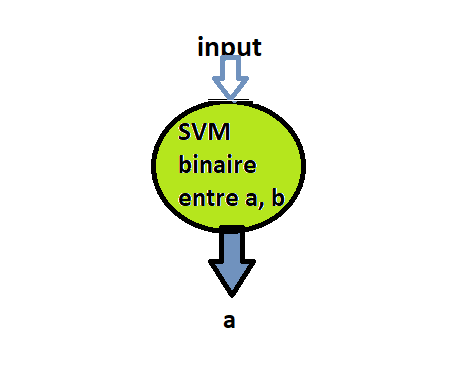
\includegraphics[scale=0.7]{Images/svm_binaire.png}
	\end{center}
	\caption{Représentation d'un modèle binaire SVM}
	\label{fig:svm0}
\end{figure}
L'algorithme utilisé consiste à faire les prédiction dans chaque modèle qu'on a , et puis après en regroupe le résultat finale dans un vecteur, qui contient lui aussi les valeurs d'apparition d'une classe dans une prédiction, on le résultat final, est la classe qui a apparu le plus, dans le vecteur .
\begin{figure}[H]
	\begin{center}
	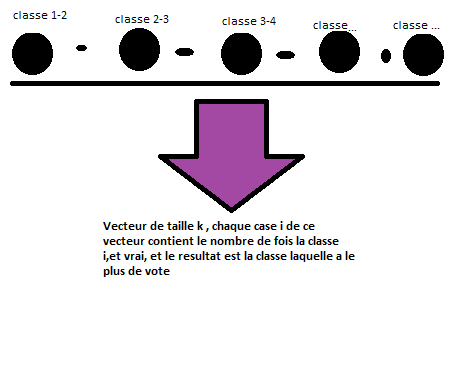
\includegraphics[scale=0.7]{Images/svm_rep.png}
	\end{center}
	\caption{Représentation globale du modèle}
	\label{fig:svm0}
\end{figure}



 L’état des pertes sur les variables de décision :

\begin{figure}[H]
	\begin{center}
	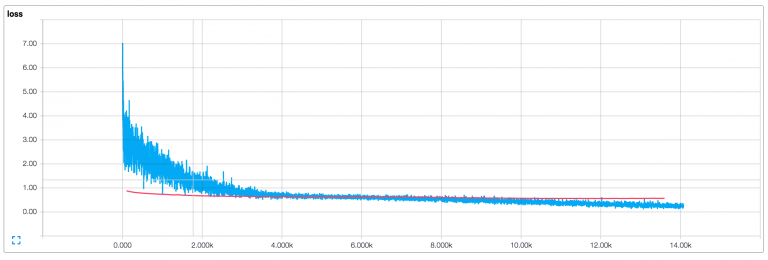
\includegraphics[width=\linewidth]{Images/cnn4.png}
	\end{center}
	\caption{Graphe qui représente les données perdues, du multiClass-SVM.}
	\label{fig:rnn}
\end{figure}
 l'état des précision qui est égale à 0,65:
\begin{figure}[H]
	\begin{center}
	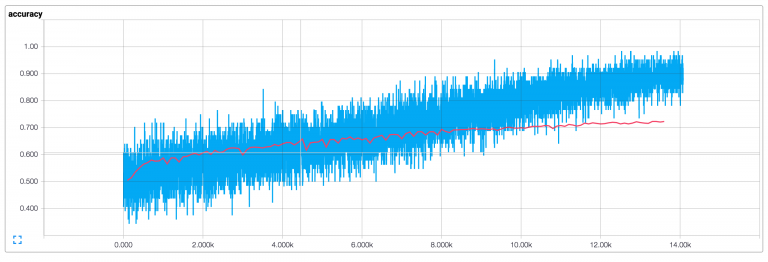
\includegraphics[width=\linewidth]{Images/cnn5.png}
	\end{center}
	\caption{Graphe qui représente la précision, du  multiClass-SVM.}
	\label{fig:rnn}
\end{figure}







\chapter{Sprint 3 : Amélioration du CNN avec word2vec}
\label{Chapitre 6} % For referencing the chapter elsewhere, use \ref{Chapter1} 

\lhead{Chapitre 6. \emph{Sprint 3 : Amélioration du CNN avec word2vec}} % This is for the header on each page - perhaps a shortened title

%----------------------------------------------------------------------------------------

\section{Spécification}
\subsection{Le Backlog du Sprint}
\begin{figure}[H]
\begin{tabular}{|p{7cm}|p{4cm}|p{4cm}|}
\hline
\textbf{Story} & \textbf{Priorité2 } & \textbf{Effort ou chargen} \\
\hline
En tant qu'utilisateur, je souhaite pouvoir visiter les différentes contenu par catégories,et de les sélectionner selon mon besoin. & \begin{center}M\end{center} & \begin{center}22\end{center}\\
\hline
\end{tabular}
  \caption{Le Backlog du Sprint 3}
  \label{fig:Backlog3}
\end{figure}
\section{Conception}
\subsection{Qu'est ce qu'un word2vec ?}
Word2vec est un groupe de modèles associés utilisés pour produire des incorporations de mots. Ces modèles sont des réseaux neuronaux à deux couches, peu profonds, formés pour reconstruire les contextes linguistiques des mots. Word2vec prend en entrée un grand corpus de texte et produit un espace vectoriel, typiquement de plusieurs centaines de dimensions, avec pour chaque mot unique du corpus un vecteur correspondant dans l'espace.\\[0.5cm]
 Les vecteurs de mots sont positionnés dans l'espace vectoriel de sorte que les mots qui partagent des contextes communs dans le corpus sont situés à proximité les uns des autres dans l'espace.\\[0.2cm]
Word2vec a été créé par une équipe de chercheurs dirigée par Tomas Mikolov chez Google. L'algorithme a ensuite été analysé et expliqué par d'autres chercheurs.  L'incorporation de vecteurs créés à l'aide de l'algorithme Word2vec présente de nombreux avantages par rapport aux algorithmes précédents tels que l'analyse sémantique latente.
\subsection{Utilisation}
Le word2vec est un réseaux neuronal, qui sert à représenter les mots par des vecteur de taille prédéfini. 



\chapter{Sprint 4 : Réalisation d’un modèle de prédiction hybride}
\label{Chapitre 7} % For referencing the chapter elsewhere, use \ref{Chapter1} 

\lhead{Chapitre 7. \emph{Sprint 4 : Réalisation d’un modèle de prédiction hybride}} % This is for the header on each page - perhaps a shortened title

%----------------------------------------------------------------------------------------

\section{Spécification}
\subsection{Le Backlog du Sprint}
\begin{figure}[H]
\begin{tabular}{|p{7cm}|p{4cm}|p{4cm}|}
\hline
\textbf{Story} & \textbf{Priorité2 } & \textbf{Effort ou chargen} \\
\hline
En tant qu'utilisateur, je souhaite pouvoir visiter les différentes contenu par catégories,et de les sélectionner selon mon besoin. & \begin{center}M\end{center} & \begin{center}22\end{center}\\
\hline
\end{tabular}
  \caption{Le Backlog du Sprint 4}
  \label{fig:Backlog4}
\end{figure}
\section{Conception}

\chapter*{Conclusion} % Main chapter title
Pour conclure, j’ai effectué mon stage de deuxième année de cycle d'ingénierie logiciel et intégration des systèmes informatique  en temps que Data Scientist pour l'application mobile Nacharat au sein de l’entreprise SanadTech. Lors de ce stage de 3 mois, j’ai pu mettre en pratique mes connaissances théoriques acquises durant ma formation et aussi ça m'a permis de m'introduire dans une nouvelle route, celle du big data et machine learning.\\[0.5cm]
Pendant cette expérience, j'ai tous d'abord traiter les données,en travailler à bien  saisir son architecture, ce qui m'a permis de les transformer en des matrices numériques, puis après j'ai commencé par aborder le problème de classification depuis le coté de deep learning en utilisant le Réseau neuronal convolutif, ce qui m'a donné une precision en dessus de la moyenne, après j'ai voulu changer l'approche de deep learning, c'est pour cela que cette fois j'ai abordé le problème  par l'une des approches du machine learning, en utilisant le Support vector machine avec un kernel gaussien, il m'a donné un résultat satisfaisant mais pas assez convaincant, et à la fin j'ai repris le premier algorithme développé, et j'ai travaillé à augmenter sa precision en utilisant le réseaux neuronal word2vec dans la phase d'entrer pour minimiser la perte des données et aussi pour données à l'algorithme d'apprendre la sémantique des mots,et tout cela pour avoir une precision bien meilleur.\\[0.5cm]
Pour le Sprint finale, j' y compte rassembler les deux approches en un seul algorithme de classification, l'algorithme va contenir une seule entrée, la première couche va contenir deux parties indépendantes le CNN plus le Word2vec et le SVM , la deuxième couche va ressembler les résultats obtenus par la première couche on un vecteur qu'on va l'analyser par la suite par la méthode de Bayes, pour enfin avoir un résultat avec un taux de precision très élevé.
%\input{Chapters/Chapter2} 
%\input{Chapters/Chapter3}
%\input{Chapters/Chapter4} 
%\input{Chapters/Chapter5} 
%\input{Chapters/Chapter6} 
%\input{Chapters/Chapter7} 

%----------------------------------------------------------------------------------------
%	THESIS CONTENT - APPENDICES
%----------------------------------------------------------------------------------------

\addtocontents{toc}{\vspace{2em}} % Add a gap in the Contents, for aesthetics

\appendix % Cue to tell LaTeX that the following 'chapters' are Appendices

% Include the appendices of the thesis as separate files from the Appendices folder
% Uncomment the lines as you write the Appendices

 %Appendix A
\chapter{CNN} % Main appendix title

% %Appendix B
%\chapter{SVM} % Main appendix title
\lhead{Annexe. \emph{SVM}} % This is for the header on each page - perhaps a shortened title
\centering{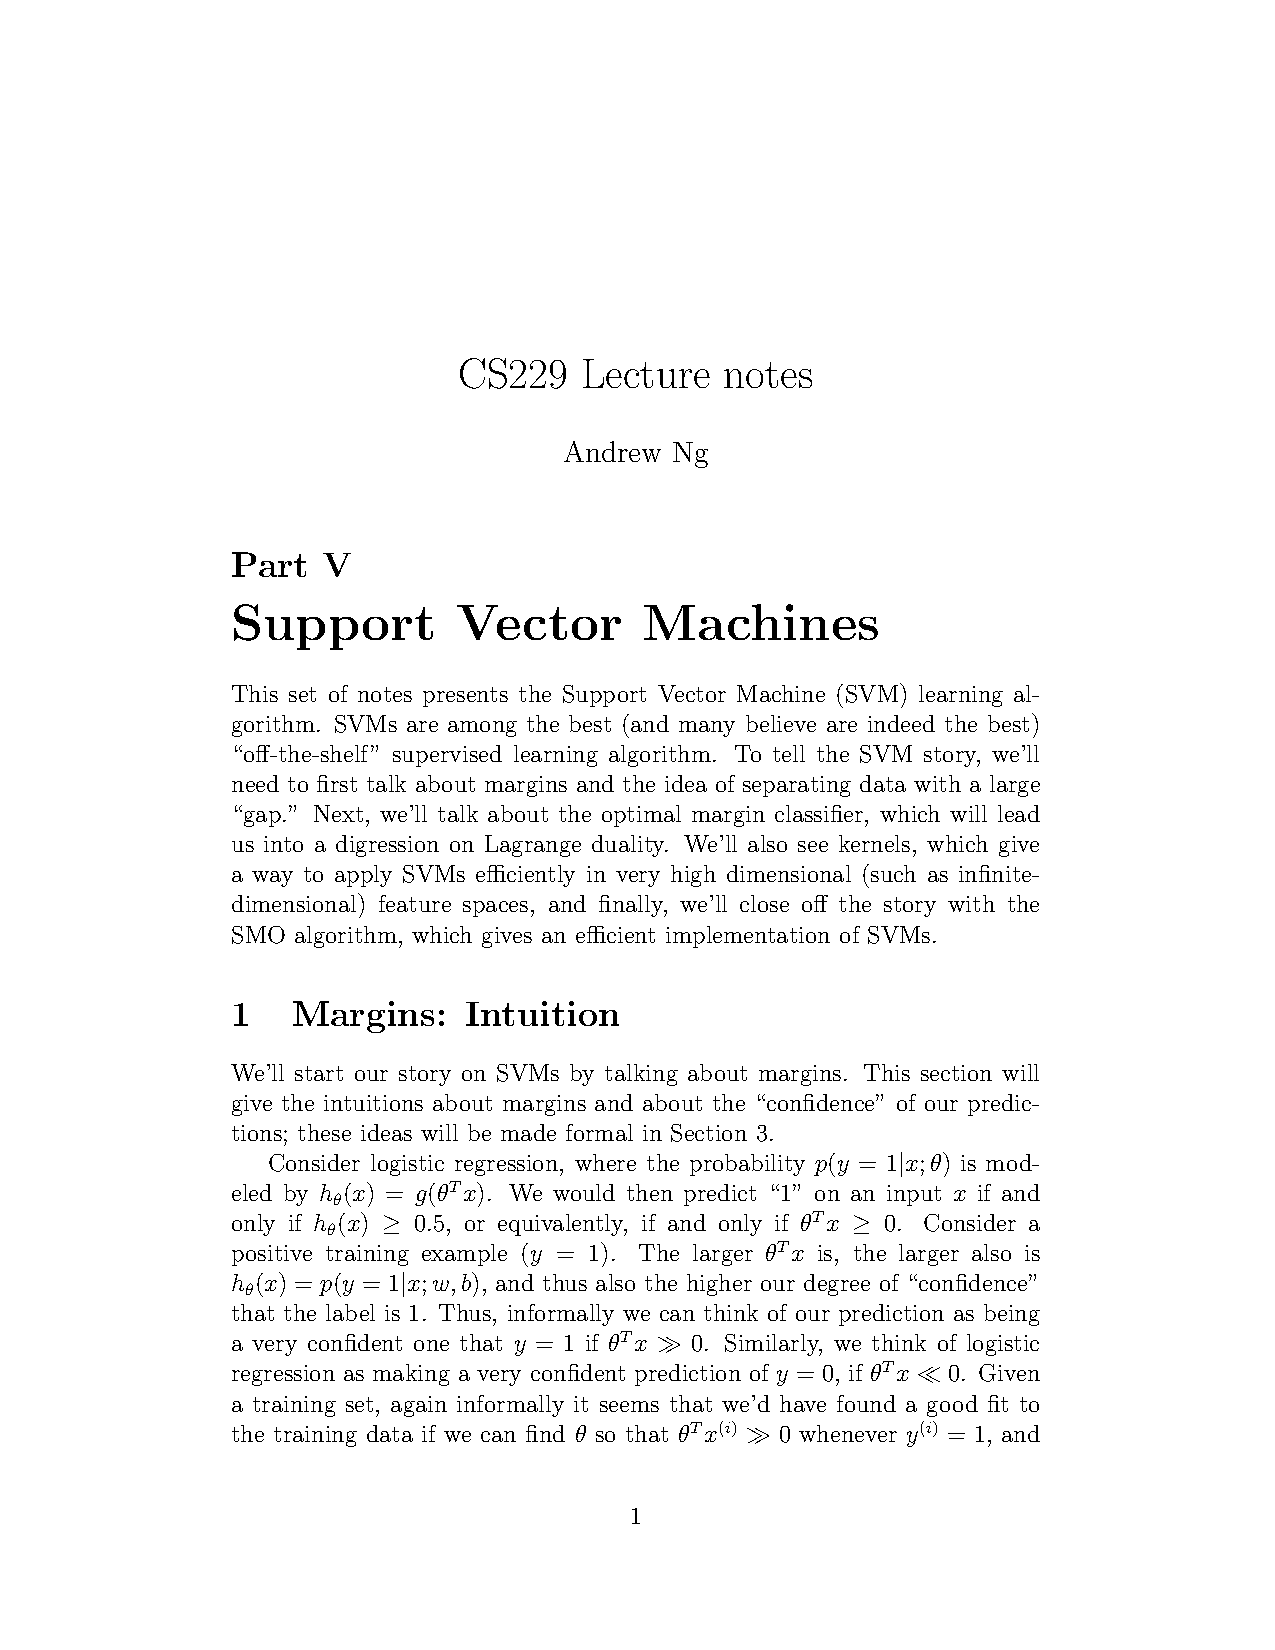
\includepdf[pages=1,width=\textwidth,pagecommand=\chapter{SVM},offset=2.5cm 0cm]{annexe2.pdf}}
\centering{\includepdf[pages=2-,width=\textwidth,pagecommand={},offset=2.5cm 0cm]{annexe2.pdf}}
% %Appendix C
%\chapter{Word2vect} % Main appendix title

\lhead{Annexe. \emph{Word2vect}} % This is for the header on each page - perhaps a shortened title

%----------------------------------------------------------------------------------------
\centering{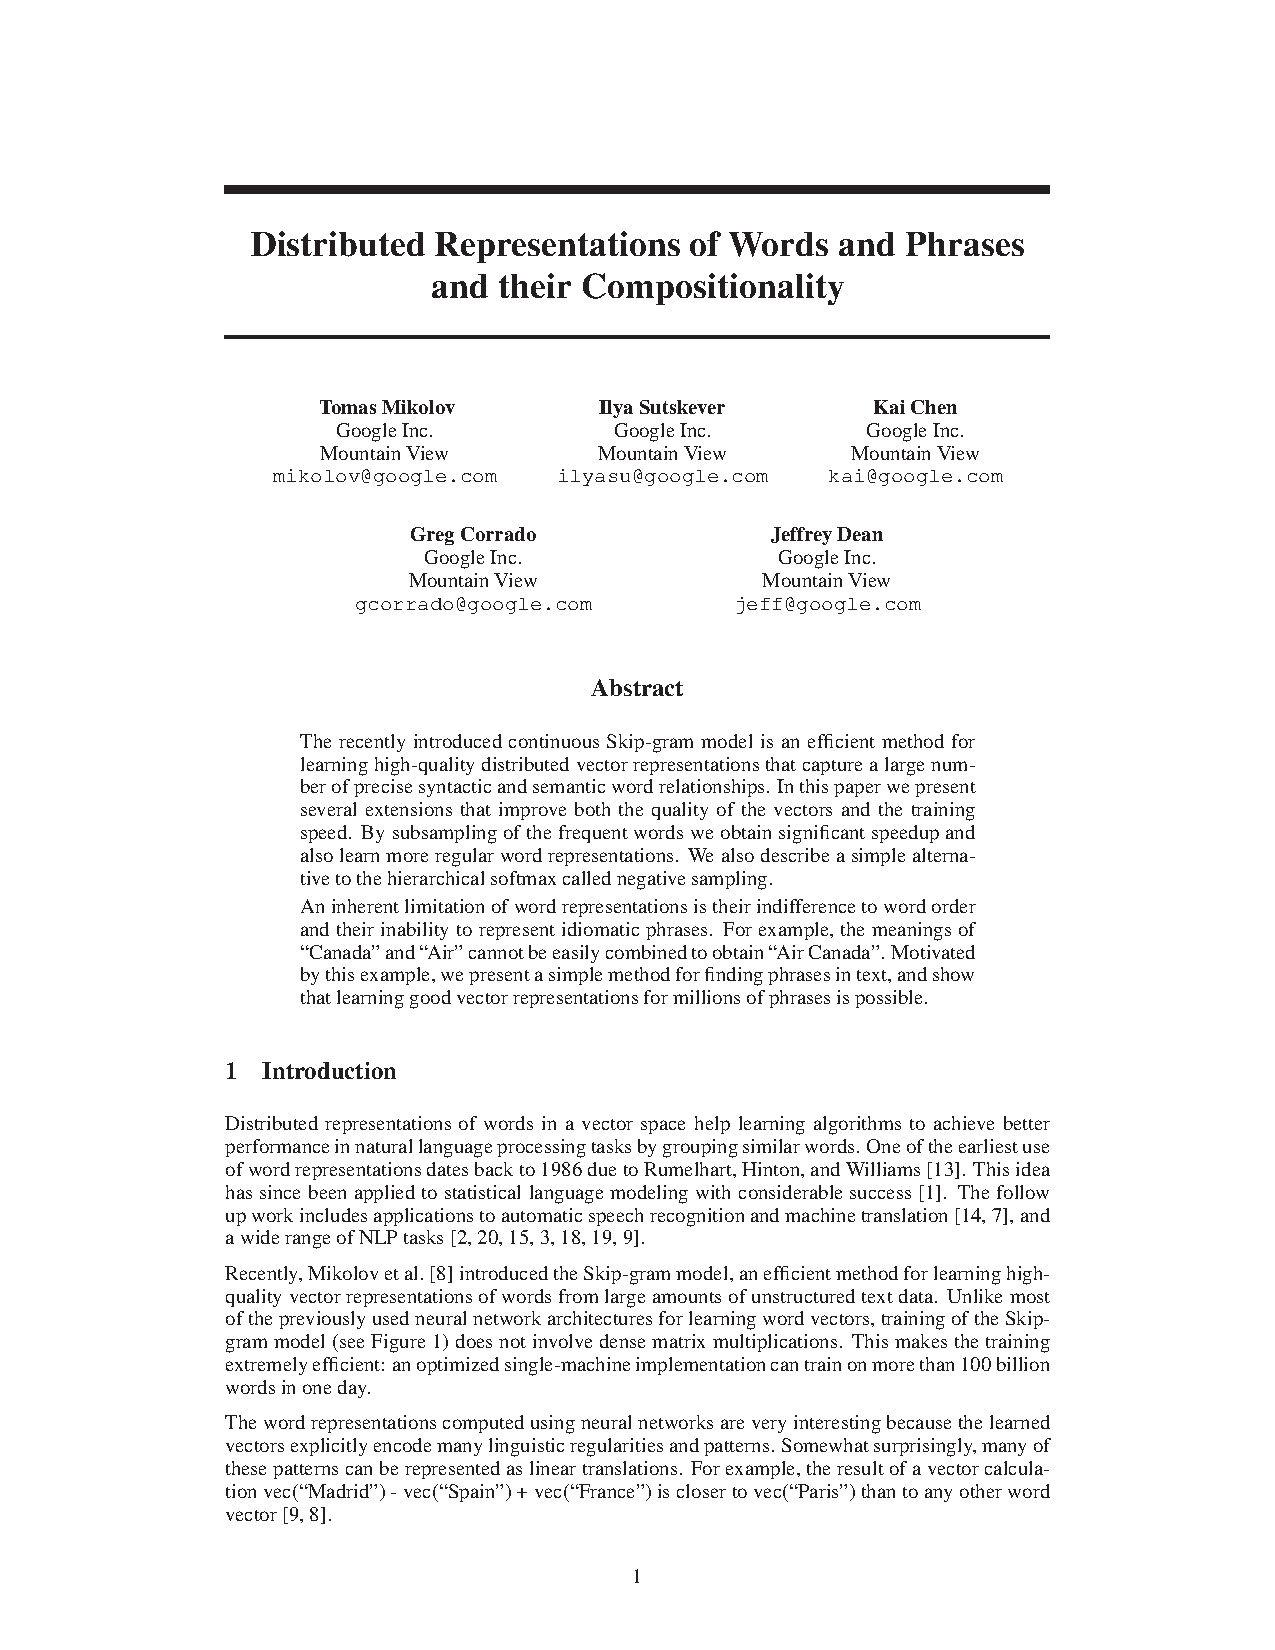
\includepdf[pages=1,width=\textwidth,pagecommand=\chapter{Word2vect},offset=2.5cm -3cm]{annexe3.pdf}}
\centering{\includepdf[pages=2-,width=\textwidth,pagecommand={},offset=2.5cm 0cm]{annexe3.pdf}}

\addtocontents{toc}{\vspace{2em}} % Add a gap in the Contents, for aesthetics

\backmatter

%----------------------------------------------------------------------------------------
%	BIBLIOGRAPHY
%----------------------------------------------------------------------------------------

\label{Bibliography}

\lhead{\emph{Bibliography}} % Change the page header to say "Bibliography"

\bibliographystyle{apalike} % Use the "apalike" BibTeX style for formatting the Bibliography

\bibliography{bibliography} % The references (bibliography) information are stored in the file named "bibliography.bib"

\end{document}